\documentclass[oneside]{book}
\usepackage[utf8]{inputenc}
\usepackage[top=1in]{geometry}
\usepackage{graphicx}
\usepackage{booktabs}
\usepackage{amsmath}
\usepackage{amsthm}
\usepackage[only]{excludeonly}
\usepackage{tikz}
\usepackage{verbatim}
\usetikzlibrary{circuits.logic.US,positioning,calc} 
\usetikzlibrary{matrix,shapes,arrows,fit,tikzmark}
\usepackage[american]{circuitikz}
\usepackage{enumitem,amssymb}
\usepackage{url}
\usepackage{wrapfig}
\usepackage[disable]{easy-todo}
\usepackage{multirow}
%\usepackage{todonotes}

% \newlist{todolist}{itemize}{2}
% \setlist[todolist]{label=$\square$}
% \usepackage{pifont}
% \newcommand{\cmark}{\ding{51}}%
% \newcommand{\xmark}{\ding{55}}%
% \newcommand{\done}{\rlap{$\square$}{\raisebox{2pt}{\large\hspace{1pt}\cmark}}%
%   \hspace{-2.5pt}}
% \newcommand{\wontfix}{\rlap{$\square$}{\large\hspace{1pt}\xmark}}

\input{0928-quine-mccluskey/karnaugh}
% Calligraphic fonts
\newcommand{\calA}{{\cal A}}
\newcommand{\calB}{{\cal B}}
\newcommand{\calC}{{\cal C}}
\newcommand{\calD}{{\cal D}}
\newcommand{\calE}{{\cal E}}
\newcommand{\calF}{{\cal F}}
\newcommand{\calG}{{\cal G}}
\newcommand{\calH}{{\cal H}}
\newcommand{\calI}{{\cal I}}
\newcommand{\calJ}{{\cal J}}
\newcommand{\calK}{{\cal K}}
\newcommand{\calL}{{\cal L}}
\newcommand{\calM}{{\cal M}}
\newcommand{\calN}{{\cal N}}
\newcommand{\calO}{{\cal O}}
\newcommand{\calP}{{\cal P}}
\newcommand{\calQ}{{\cal Q}}
\newcommand{\calR}{{\cal R}}
\newcommand{\calS}{{\cal S}}
\newcommand{\calT}{{\cal T}}
\newcommand{\calU}{{\cal U}}
\newcommand{\calV}{{\cal V}}
\newcommand{\calW}{{\cal W}}
\newcommand{\calX}{{\cal X}}
\newcommand{\calY}{{\cal Y}}
\newcommand{\calZ}{{\cal Z}}

% Sets:
\newcommand{\setA}{\textsf{A}}
\newcommand{\setB}{\textsf{B}}
\newcommand{\setC}{\textsf{C}}
\newcommand{\setD}{\textsf{D}}
\newcommand{\setE}{\textsf{E}}
\newcommand{\setF}{\textsf{F}}
\newcommand{\setG}{\textsf{G}}
\newcommand{\setH}{\textsf{H}}
\newcommand{\setI}{\textsf{I}}
\newcommand{\setJ}{\textsf{J}}
\newcommand{\setK}{\textsf{K}}
\newcommand{\setL}{\textsf{L}}
\newcommand{\setM}{\textsf{M}}
\newcommand{\setN}{\textsf{N}}
\newcommand{\setO}{\textsf{O}}
\newcommand{\setP}{\textsf{P}}
\newcommand{\setQ}{\textsf{Q}}
\newcommand{\setR}{\textsf{R}}
\newcommand{\setS}{\textsf{S}}
\newcommand{\setT}{\textsf{T}}
\newcommand{\setU}{\textsf{U}}
\newcommand{\setV}{\textsf{V}}
\newcommand{\setW}{\textsf{W}}
\newcommand{\setX}{\textsf{X}}
\newcommand{\setY}{\textsf{Y}}
\newcommand{\setZ}{\textsf{Z}}

% Vectors
\newcommand{\bfa}{\mathbf{a}}
\newcommand{\bfb}{\mathbf{b}}
\newcommand{\bfc}{\mathbf{c}}
\newcommand{\bfd}{\mathbf{d}}
\newcommand{\bfe}{\mathbf{e}}
\newcommand{\bff}{\mathbf{f}}
\newcommand{\bfg}{\mathbf{g}}
\newcommand{\bfh}{\mathbf{h}}
\newcommand{\bfi}{\mathbf{i}}
\newcommand{\bfj}{\mathbf{j}}
\newcommand{\bfk}{\mathbf{k}}
\newcommand{\bfl}{\mathbf{l}}
\newcommand{\bfm}{\mathbf{m}}
\newcommand{\bfn}{\mathbf{n}}
\newcommand{\bfo}{\mathbf{o}}
\newcommand{\bfp}{\mathbf{p}}
\newcommand{\bfq}{\mathbf{q}}
\newcommand{\bfr}{\mathbf{r}}
\newcommand{\bfs}{\mathbf{s}}
\newcommand{\bft}{\mathbf{t}}
\newcommand{\bfu}{\mathbf{u}}
\newcommand{\bfv}{\mathbf{v}}
\newcommand{\bfw}{\mathbf{w}}
\newcommand{\bfx}{\mathbf{x}}
\newcommand{\bfy}{\mathbf{y}}
\newcommand{\bfz}{\mathbf{z}}


\newcommand{\bfalpha}{\boldsymbol{\alpha}}
\newcommand{\bfbeta}{\boldsymbol{\beta}}
\newcommand{\bfgamma}{\boldsymbol{\gamma}}
\newcommand{\bfdelta}{\boldsymbol{\delta}}
\newcommand{\bfepsilon}{\boldsymbol{\epsilon}}
\newcommand{\bfzeta}{\boldsymbol{\zeta}}
\newcommand{\bfeta}{\boldsymbol{\eta}}
\newcommand{\bftheta}{\boldsymbol{\theta}}
\newcommand{\bfiota}{\boldsymbol{\iota}}
\newcommand{\bfkappa}{\boldsymbol{\kappa}}
\newcommand{\bflambda}{\boldsymbol{\lambda}}
\newcommand{\bfmu}{\boldsymbol{\mu}}
\newcommand{\bfnu}{\boldsymbol{\nu}}
\newcommand{\bfomicron}{\boldsymbol{\omicron}}
\newcommand{\bfpi}{\boldsymbol{\pi}}
\newcommand{\bfrho}{\boldsymbol{\rho}}
\newcommand{\bfsigma}{\boldsymbol{\sigma}}
\newcommand{\bftau}{\boldsymbol{\tau}}
\newcommand{\bfupsilon}{\boldsymbol{\upsilon}}
\newcommand{\bfphi}{\boldsymbol{\phi}}
\newcommand{\bfchi}{\boldsymbol{\chi}}
\newcommand{\bfpsi}{\boldsymbol{\psi}}
\newcommand{\bfomega}{\boldsymbol{\omega}}
\newcommand{\bfxi}{\boldsymbol{\xi}}
\newcommand{\bfell}{\boldsymbol{\ell}}

% Matrices
\newcommand{\bfA}{\mathbf{A}}
\newcommand{\bfB}{\mathbf{B}}
\newcommand{\bfC}{\mathbf{C}}
\newcommand{\bfD}{\mathbf{D}}
\newcommand{\bfE}{\mathbf{E}}
\newcommand{\bfF}{\mathbf{F}}
\newcommand{\bfG}{\mathbf{G}}
\newcommand{\bfH}{\mathbf{H}}
\newcommand{\bfI}{\mathbf{I}}
\newcommand{\bfJ}{\mathbf{J}}
\newcommand{\bfK}{\mathbf{K}}
\newcommand{\bfL}{\mathbf{L}}
\newcommand{\bfM}{\mathbf{M}}
\newcommand{\bfN}{\mathbf{N}}
\newcommand{\bfO}{\mathbf{O}}
\newcommand{\bfP}{\mathbf{P}}
\newcommand{\bfQ}{\mathbf{Q}}
\newcommand{\bfR}{\mathbf{R}}
\newcommand{\bfS}{\mathbf{S}}
\newcommand{\bfT}{\mathbf{T}}
\newcommand{\bfU}{\mathbf{U}}
\newcommand{\bfV}{\mathbf{V}}
\newcommand{\bfW}{\mathbf{W}}
\newcommand{\bfX}{\mathbf{X}}
\newcommand{\bfY}{\mathbf{Y}}
\newcommand{\bfZ}{\mathbf{Z}}


\newcommand{\bfGamma}{\boldsymbol{\Gamma}}
\newcommand{\bfDelta}{\boldsymbol{\Delta}}
\newcommand{\bfTheta}{\boldsymbol{\Theta}}
\newcommand{\bfLambda}{\boldsymbol{\Lambda}}
\newcommand{\bfPi}{\boldsymbol{\Pi}}
\newcommand{\bfSigma}{\boldsymbol{\Sigma}}
\newcommand{\bfUpsilon}{\boldsymbol{\Upsilon}}
\newcommand{\bfPhi}{\boldsymbol{\Phi}}
\newcommand{\bfPsi}{\boldsymbol{\Psi}}
\newcommand{\bfOmega}{\boldsymbol{\Omega}}


% Blackboard Bold:
\newcommand{\bbA}{\mathbb{A}}
\newcommand{\bbB}{\mathbb{B}}
\newcommand{\bbC}{\mathbb{C}}
\newcommand{\bbD}{\mathbb{D}}
\newcommand{\bbE}{\mathbb{E}}
\newcommand{\bbF}{\mathbb{F}}
\newcommand{\bbG}{\mathbb{G}}
\newcommand{\bbH}{\mathbb{H}}
\newcommand{\bbI}{\mathbb{I}}
\newcommand{\bbJ}{\mathbb{J}}
\newcommand{\bbK}{\mathbb{K}}
\newcommand{\bbL}{\mathbb{L}}
\newcommand{\bbM}{\mathbb{M}}
\newcommand{\bbN}{\mathbb{N}}
\newcommand{\bbO}{\mathbb{O}}
\newcommand{\bbP}{\mathbb{P}}
\newcommand{\bbQ}{\mathbb{Q}}
\newcommand{\bbR}{\mathbb{R}}
\newcommand{\bbS}{\mathbb{S}}
\newcommand{\bbT}{\mathbb{T}}
\newcommand{\bbU}{\mathbb{U}}
\newcommand{\bbV}{\mathbb{V}}
\newcommand{\bbW}{\mathbb{W}}
\newcommand{\bbX}{\mathbb{X}}
\newcommand{\bbY}{\mathbb{Y}}
\newcommand{\bbZ}{\mathbb{Z}}




\graphicspath{{0831-number-system/}
{0831-number-system}
{0907-boolean-algebra}
{0916-K-maps}
{homeworks/hw1}
{homeworks/hw2}
{labs/01-quartus-setup/}
 {labs/02-verilog-mux/}
{0928-adders-carry-ahead}
{0928-quine-mccluskey}
{0930-review}
{1014-analog-details}
{1024-cmos-gate-review}
{1026-sequential-logic}
{1031-review}
{1121-mealy-moore-seq-detector}
{11-29-notes.pdf}
{1130-FSM-optimization}
{1205-mux-decoder}
{1207-more-definitions}
} 
\title{Digital circuit design notes}
\author{Vikas Dhiman for ECE275\footnote{The notes are from the following books \cite{harris2022digital,stephen2022fundamentals}. Not intended for distribution outside the class.}}
\newtheorem{example}{Example}[chapter]
\newtheorem{prob}{Problem}[chapter]
\newtheorem{remark}{Remark}[chapter]
\newtheorem{definition}{Definition}[chapter]

\newcommand{\bw}{\bar{w}}
\newcommand{\bx}{\bar{x}}
\newcommand{\by}{\bar{y}}
\newcommand{\bz}{\bar{z}}
\newcommand{\bW}{\bar{W}}
\newcommand{\bX}{\bar{X}}
\newcommand{\bY}{\bar{Y}}
\newcommand{\bZ}{\bar{Z}}
\newcommand{\bA}{\bar{A}}
\newcommand{\bB}{\bar{B}}
\newcommand{\bC}{\bar{C}}
\newcommand{\bD}{\bar{D}}

\newcommand{\cred}{\color{red}}
\newcommand{\cg}{\color{green!60!black}}
\newcommand{\cb}{\color{blue}}
% Some options common to all the nodes and paths
\tikzset{   
  every picture/.style={remember picture,baseline},
  every node/.style={anchor=base,align=center,outer sep=1.5pt},
  every path/.style={thick},
}

\newcommand\marktopleft[1]{%
  \tikz[overlay,remember picture] 
  \node (marker-#1-a) at (.3em,.3em) {};%
}
\newcommand\markbottomright[2]{%
  \tikz[overlay,remember picture] 
  \node (marker-#1-b) at (.1em,.3em) {};%
  \tikz[overlay,remember picture,inner sep=1pt]
  \node[draw={#2},rounded corners,fit=(marker-#1-a.north west) (marker-#1-b.south east)] {};%
}
\newcommand\markpolytopleft[1]{%
  \tikz[overlay,remember picture]%
  \node (marker-#1-tl) at (.3em,.3em) {};%
}
\newcommand\markpolytopright[1]{%
  \tikz[overlay,remember picture]%
  \node (marker-#1-tr) at (.3em,.3em) {};%
}
\newcommand\markpolybottomright[1]{%
  \tikz[overlay,remember picture] 
  \node (marker-#1-br) at (.3em,.3em) {};%
  }
\newcommand\markpolybottomleft[2]{%
  \tikz[overlay,remember picture]
  \node (marker-#1-bl) at (.3em,.3em) {};%
  \tikz[overlay,remember picture,inner sep=1pt]
  \path [draw={#2},rounded corners]
  (marker-#1-tl.north west) --
  (marker-#1-tl.north east) --
  (marker-#1-bl.south east) --
  (marker-#1-br.south west);%
}

\newcommand{\notescol}{black}

\input{labs/01-quartus-setup/lab-preamble.tex}

\begin{document}
\maketitle

\tableofcontents
\newpage
\listoftodos

\todoi{Weave homeworks, labs and notes}
\todoi{Less emphasis on K-maps, more on Verilog}
\todoi{Maybe quine mccluskey and espresso by C-coding example}

\newpage


\chapter{Boolean Algebra}
\maketitle
\section{Learning objectives}
\begin{enumerate}
\item Representing digital circuits
\item Converting between different notations: Boolean expression, logic
  networks and switching circuits
\item Converting between different logic network specifications: truth table, minterm,
  maxterms, product of sums canonical form and sum of product canonical form.
\item Introduce truth tables as Behavioral Verilog
\item This handout has 11 homework problems totaling to 140 marks
\end{enumerate}

\section{Motivating Problem}

\begin{example}
  Assume that a large room has three doors and that a switch near each door controls a light in the room. It has to be possible to turn the light on or off by changing the state of any one
  of the switches.\\
  \includegraphics[width=\linewidth]{figures/design-a-3-way-light-switch.pdf}
\end{example}

\rotatebox[origin=c]{90}{
\begin{tabular}{lccp{0.2\linewidth}ccc}
  \toprule
  Name & C/Verilog & Boolean expr. & Truth Table & Switching circuit & (ANSI) symbol & Venn diagram  \\
  \midrule
  AND Gate &
  \texttt{L = x1 \& x2} &
  $L = x_1 \cdot x_2 = x_1 x_2$ &
 \mbox{\begin{tabular}{cc|c}
 \toprule
 $x_1$ & $x_2$ & $x_1 \cdot x_2$ \\
 \midrule
 0 & 0 & 0 \\
 0 & 1 & 0 \\
 1 & 0 & 0 \\
 1 & 1 & 1 \\
 \bottomrule
 \end{tabular}} &
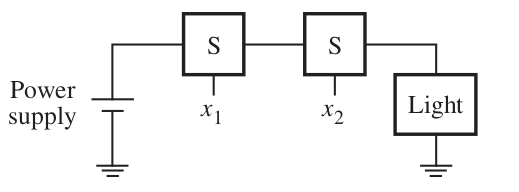
\includegraphics[width=0.2\linewidth]{AND-circuit.png} &
\includegraphics[width=0.2\linewidth]{AND_ANSI.pdf} &
\includegraphics[width=0.2\linewidth]{AND_Venn.pdf}\\
  OR Gate &
\texttt{L = x1 | x2} &
$L = x_1 + x_2$ &
\mbox{\begin{tabular}{cc|c}
  \toprule
  $x_1$ & $x_2$ & $x_1 + x_2$ \\
  \midrule
  0 & 0 & 0 \\
  0 & 1 & 1 \\
  1 & 0 & 1 \\
  1 & 1 & 1 \\
  \bottomrule
\end{tabular}} &
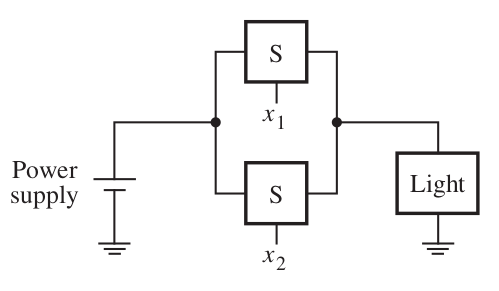
\includegraphics[width=0.2\linewidth]{OR-circuit.png} &
\includegraphics[width=0.2\linewidth]{OR_ANSI.pdf} & 
\includegraphics[width=0.2\linewidth]{OR_Venn.pdf}\\
  NOT Gate &
  \texttt{L = $\sim$ x1} &
$ L = \bar{x}_1 = x'_1$ &
\mbox{\begin{tabular}{c|c}
\toprule
$x_1$ & $\bar{x}_1$ \\
\midrule
0 & 1 \\
1 & 0 \\
\bottomrule
\end{tabular}} &
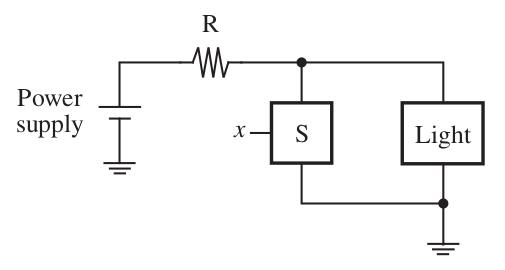
\includegraphics[width=0.2\linewidth]{NOT-circuit.png} &
\includegraphics[width=0.2\linewidth]{NOT_ANSI.pdf} &
\includegraphics[width=0.2\linewidth]{NOT_Venn_x1.pdf}
\end{tabular}
}
\newpage

\section{Digital circuits or networks}

\begin{tikzpicture}[circuit logic US]
    \node (A) at (0,1) {A} ;
    \node (B) at (0,0.5) {B} ;
    \node (C) at (0,0) {C} ;
    \node [draw,rounded corners,inner sep=7mm,anchor=south west] (CL) at (1, -3mm) {CL} ; 
    \node [above right=3mm of CL.east] (Y) {Y} ;
    \node [below right=3mm of CL.east] (Z) {Z} ;

    \draw (A) -| (CL.west);
    \draw (B) -| (CL.west);
    \draw (C) -| (CL.west);
    \draw (CL.east) |- (Y);
    \draw (CL.east) |- (Z);
\end{tikzpicture}

\[
  Y = F(A, B, C) \qquad Z = G(A, B, C)
  \]

\section{Two input networks}
\begin{example}
  Convert the following (ANSI) network into a Boolean expression, a truth table
  and a Venn diagram.

\begin{tikzpicture}[circuit logic US]
  \matrix[column sep=7mm]{
    \node (i1) {$x_1$}; & &  \\
    & \node [and gate] (a) {}; & \node [not gate] (n) {};\\
    \node (i2) {$x_2$}; & &  \\
  };
  \draw (i1.east) -- ++(right:3mm) |- (a.input 1);
  \draw (i2.east) -- ++(right:3mm) |- (a.input 2);
  \draw (a.output) to [edge label=g] (n.input);
  \draw (n.output) to [edge label=f] ++(right:3mm);
\end{tikzpicture}
\end{example}
\vspace{10em}

\begin{example}
  Convert the following Boolean expression into a (ANSI) network, a truth
  table and a Venn diagram:\\
  \[ f = \overline{x_1 + x_2}\]
\end{example}
\vspace{10em}

\begin{prob}[10 marks]
  Convert the following (ANSI) network into a Boolean expression, a truth table
  and a Venn diagram.

 \noindent \begin{tikzpicture}[circuit logic US]
    \matrix[column sep=7mm]{
      \node (i1) {$x_1$}; & & \node [and gate] (x1nx2) {}; & \\
      \node (i2) {$x_2$}; &  &  &  \node [or gate] (f) {}; \\
       & \node [not gate] (n1) {}; & \node [and gate] (nx1x2) {};&  \\
      & \node [not gate] (n2) {}; &  & \\
    };
    \draw (i1.east) -- ++(right:4mm) |- (n1.input);
    \draw (i2.east) -- ++(right:2mm) |- (n2.input);

    \draw (i1.east) -- ++(right:4mm) |- (x1nx2.input 1);
    \draw (i2.east) -- ++(right:2mm) |- (x1nx2.input 2);

    \draw (n1.output) -- ++(right:3mm) |- (nx1x2.input 1);
    \draw (n2.output) -- ++(right:3mm) |- (nx1x2.input 2);

    \draw (x1nx2.output) -- ++(right:3mm) |- (f.input 1);
    \draw (nx1x2.output) -- ++(right:3mm) |- (f.input 2);

    \draw (f.output) to [edge label=f] ++(right:3mm);
  \end{tikzpicture}
\end{prob}
\vspace{10em}

\begin{example}
  Convert the following Boolean expression into a network, a truth
  table and a Venn diagram:\\
  \[ f = x_1 \bar{x}_2 + \bar{x}_1 x_2 \]
\end{example}
\vspace{20em}

\begin{prob}[5 marks]
Can two different circuits have the same truth table? Can two different truth tables
have the same circuit? Consider the following two circuits for example \\
\noindent\begin{tikzpicture}[circuit logic US]
  \node (A) {A}; \node [not gate, right=of A] (notA) {}; \node [right=of notA] (Y) {Y};
  \draw (A) -- (notA.input);
  \draw (notA.output) -- (Y);
\end{tikzpicture}\\[1em]

\noindent\begin{tikzpicture}[circuit logic US]
  \node (A) {A}; \node [not gate, right=of A] (notA1) {};
  \draw (A) -- (notA.input);

  \node [not gate, right=of notA1] (notA2) {};
  \draw (notA1.output) -- (notA2.input);

  \node [not gate, right=of notA2] (notA3) {};
  \draw (notA2.output) -- (notA3.input);

  \node [right=of notA3] (Y) {Y};
  \draw (notA3.output) -- (Y);
\end{tikzpicture}

%How about Venn diagrams?
\end{prob}
\vspace{10em}

\begin{remark}
  Truth tables and Venn diagrams define \emph{what} the combinational circuit should do. Truth tables
  define output for every input.
  Boolean expression and networks define \emph{how} to achieve the desired input
  output relationship.
\end{remark}


\section{Multi-input networks}
\begin{example}
  Convert the following (ANSI) network into a Boolean expression and a truth table.
  \begin{tikzpicture}[circuit logic US]
    \matrix[column sep=7mm]{
      \node (A) {$A$}; & &  \node [and gate] (andAB) {}; & & & \\
      \node (B) {$B$}; & \node [not gate] (nB) {};  &  & \node [or gate] (orGC) {}; & \node [not gate] (notH) {}; & \\
      \node (C) {$C$}; & & \node (C2) {}; & & & \node [and gate] (andHD) {}; \\
      \node (D) {$D$}; & &  & & \node (D2) {}; &\\
    };
    \draw (A) -- ++(right:3mm) |- (andAB.input 1);
    \draw (B) -- (nB.input);
    \draw (nB.output) -- ++(right:3mm) |- (andAB.input 2);

    \draw (andAB.output) to [edge label=g] ++(right:3mm) |- (orGC.input 1);
    \draw (C) -- (C2.east) -- ++(right:3mm) |- (orGC.input 2);

    \draw (orGC.output)  to [edge label=h] (notH.input);

    \draw (notH.output) -- ++(right:3mm) |- (andHD.input 1);
    \draw (D) -- (D2.east) -- ++(right:3mm) |- (andHD.input 2);
    
    \draw (andHD.output) to [edge label=f] ++(right:3mm);
  \end{tikzpicture}
\end{example}
\vspace{20em}

\begin{prob}[20 marks]
  Convert the following (ANSI) network into a Boolean expression and a truth table.
  \begin{tikzpicture}[circuit logic US]
    \matrix[column sep=7mm]{
      \node (A) {$A$}; & &  \node [or gate] (andAB) {}; & & & \\
      \node (B) {$B$}; & \node [not gate] (nB) {};  &  & \node [and gate] (orGC) {}; &  & \\
      \node (C) {$C$}; & & \node (C2) {}; & & & \node [and gate] (andHD) {}; \\
      \node (D) {$D$}; & &  & & \node (D2) {}; &\\
    };
    \draw (A) -- ++(right:3mm) |- (andAB.input 1);
    \draw (B) -- (nB.input);
    \draw (nB.output) -- ++(right:3mm) |- (andAB.input 2);

    \draw (andAB.output) to [edge label=g] ++(right:3mm) |- (orGC.input 1);
    \draw (C) -- (C2.east) -- ++(right:3mm) |- (orGC.input 2);

    %\draw (orGC.output)  to [edge label=h] (andHD.input);

    \draw (orGC.output) to [edge label=h] ++(right:3mm) |- (andHD.input 1);
    \draw (D) -- (D2.east) -- ++(right:3mm) |- (andHD.input 2);
    
    \draw (andHD.output) to [edge label=f] ++(right:3mm);
  \end{tikzpicture}
\end{prob}
\vspace{20em}

\section{Minterms and Maxterms}
\subsection{Minterms}
Minterm is a product involving all inputs (or complements) to a function.
Every row of a truth table has a corresponding minterm.
Minterm is true if and only if the corresponding row in the table is active.

Minterms defined as follows for each row of a two input truth table:\\
\begin{tabular}{rrrp{20mm}}
  \toprule
  A & B &  minterm & minterm name\\
  \midrule
  0 & 0 &  $\bar{A} \bar{B}$ & $m_0$ \\
  0 & 1 &  $\bar{A}      B $ & $m_1$ \\
  1 & 0 &  $     A  \bar{B}$ & $m_2$ \\
  1 & 1 &  $     A       B $ & $m_3$ \\
  \bottomrule
\end{tabular}\\[1em]

\noindent Consider a two input circuit whose output $Y$ is given by the truth table:\\
\begin{tabular}{rrrrp{20mm}}
  \toprule
  A & B &  Y & minterm & minterm name\\
  \midrule
  0 & 0 & 0 & $\bar{A} \bar{B}$ & $m_0$ \\
  0 & 1 & 1 & $\bar{A}      B $ & $m_1$ \\
  1 & 0 & 0 & $     A  \bar{B}$ & $m_2$ \\
  1 & 1 & 1 & $     A       B $ & $m_3$ \\
  \bottomrule
\end{tabular}\\[1em]
then $Y = \bar{A}      B  + A B = m_1 + m_3 = \sum (1, 3)$.

\noindent This also gives the \emph{sum of products canonical form}.

\begin{example}
  What is the minterm $m_{13}$ for a 4-input circuit with inputs $x, y, z, w$
  (ordered from MSB to LSB).
\end{example}
\vspace{10em}

%\noindent Find the minterm $m_n$
%\begin{enumerate}
%    \item Convert the minterm number $n$ to a $m$-bit binary number where $m$ is the
%      order of inputs.
%    \item Replace 0 with the corresponding input complement and 1 with the input.
%\end{enumerate}

\begin{prob}[5 marks]
  What is the minterm $m_{23}$ for a 5-input circuit with inputs $a, b, c, d, e$
  (ordered from MSB to LSB).
\end{prob}
\vspace{10em}

\begin{example}
  Convert the following 4-input truth table into sum of minterms and sum of products canonical form.

  \noindent \begin{tabular}{p{20mm}llll|l}
    \toprule
    minterm name & A & B & C & D & f \\
    \midrule
    $m_0$ & 0 & 0 & 0 & 0 & 0 \\ 
    $m_1$ & 0 & 0 & 0 & 1 & 1 \\ 
    $m_2$ & 0 & 0 & 1 & 0 & 0 \\ 
    $m_3$ & 0 & 0 & 1 & 1 & 0 \\ 
    $m_4$ & 0 & 1 & 0 & 0 & 0 \\ 
    $m_5$ & 0 & 1 & 0 & 1 & 1 \\ 
    $m_6$ & 0 & 1 & 1 & 0 & 0 \\ 
    $m_7$ & 0 & 1 & 1 & 1 & 0 \\ 
    $m_8$ & 1 & 0 & 0 & 0 & 0 \\ 
    $m_9$ & 1 & 0 & 0 & 1 & 0 \\ 
    $m_{10}$ & 1 & 0 & 1 & 0 & 0 \\
    $m_{11}$ & 1 & 0 & 1 & 1 & 0 \\
    $m_{12}$ & 1 & 1 & 0 & 0 & 0 \\
    $m_{13}$ & 1 & 1 & 0 & 1 & 1 \\
    $m_{14}$ & 1 & 1 & 1 & 0 & 0 \\
    $m_{15}$ & 1 & 1 & 1 & 1 & 0 \\
    \bottomrule
  \end{tabular}
\end{example}

\begin{prob}[10 marks]
  Convert the following 4-input truth table into sum of minterms and sum of products canonical form.

  \noindent
  \begin{tabular}{p{20mm}llll|l}
    \toprule
    minterm name & A & B & C & D & f \\
    \midrule
    $m_0$ & 0 & 0 & 0 & 0 & 0 \\ 
    $m_1$ & 0 & 0 & 0 & 1 & 0 \\ 
    $m_2$ & 0 & 0 & 1 & 0 & 0 \\ 
    $m_3$ & 0 & 0 & 1 & 1 & 1 \\ 
    $m_4$ & 0 & 1 & 0 & 0 & 0 \\ 
    $m_5$ & 0 & 1 & 0 & 1 & 0 \\ 
    $m_6$ & 0 & 1 & 1 & 0 & 0 \\ 
    $m_7$ & 0 & 1 & 1 & 1 & 1 \\ 
    $m_8$ & 1 & 0 & 0 & 0 & 0 \\ 
    $m_9$ & 1 & 0 & 0 & 1 & 0 \\ 
    $m_{10}$ & 1 & 0 & 1 & 0 & 0 \\
    $m_{11}$ & 1 & 0 & 1 & 1 & 1 \\
    $m_{12}$ & 1 & 1 & 0 & 0 & 0 \\
    $m_{13}$ & 1 & 1 & 0 & 1 & 1 \\
    $m_{14}$ & 1 & 1 & 1 & 0 & 1 \\
    $m_{15}$ & 1 & 1 & 1 & 1 & 0 \\
    \bottomrule
  \end{tabular}
\end{prob}


\subsection{Maxterms}
Maxterm is a sum involving all inputs (or complements) to a function.
Every row of a truth table has a corresponding maxterm.
Minterm is false if and only if the corresponding row in the table is active.

Maxterms are defined as follows for each row of a two input truth table:\\
\begin{tabular}{rrrp{20mm}}
  \toprule
  A & B &  maxterm & maxterm name\\
  \midrule
  0 & 0 &  $A + B$ & $M_0$ \\
  0 & 1 &  $A + \bar{B} $ & $M_1$ \\
  1 & 0 &  $\bar{A} + B$ & $M_2$ \\
  1 & 1 &  $\bar{A} + \bar{B} $ & $M_3$ \\
  \bottomrule
\end{tabular}\\[1em]

\noindent Consider a two input circuit whose output $Y$ is given by the truth table:\\
\begin{tabular}{rrrrp{20mm}}
  \toprule
  A & B &  Y & maxterm & maxterm name\\
  \midrule
  0 & 0 &  0 & $A + B$ & $M_0$ \\
  0 & 1 &  1 & $A + \bar{B} $ & $M_1$ \\
  1 & 0 &  0 & $\bar{A} + B$ & $M_2$ \\
  1 & 1 &  1 & $\bar{A} + \bar{B} $ & $M_3$ \\
  \bottomrule
\end{tabular}\\[1em]
then $Y = (A+B)(\bar{A} + B) = M_0M_2$.

\noindent Writing a functional specification in terms of minterms is also called
product of sums canonical form.

\begin{example}
  Write the maxterm $M_{11}$ for 4-input Boolean function with the ordered inputs $A, B, C, D$.
\end{example}

% \noindent Find the maxterm $M_n$
% \begin{enumerate}
% \item Convert the maxterm number $n$ to a $m$-bit binary number where $m$ is the
%   order of inputs.
% \item Replace 0 with the corresponding input and 1 with the input complement.
% Add + between each input.
% \end{enumerate}

\begin{example}
  Convert the following 4-input truth table into product of maxterms and product of sums canonical form.

  \noindent
  \begin{tabular}{p{20mm}llll|l}
    \toprule
    maxterm name & A & B & C & D & f \\
    \midrule
    $M_0$ & 0 & 0 & 0 & 0 & 0 \\ 
    $M_1$ & 0 & 0 & 0 & 1 & 0 \\ 
    $M_2$ & 0 & 0 & 1 & 0 & 0 \\ 
    $M_3$ & 0 & 0 & 1 & 1 & 1 \\ 
    $M_4$ & 0 & 1 & 0 & 0 & 0 \\ 
    $M_5$ & 0 & 1 & 0 & 1 & 0 \\ 
    $M_6$ & 0 & 1 & 1 & 0 & 0 \\ 
    $M_7$ & 0 & 1 & 1 & 1 & 1 \\ 
    $M_8$ & 1 & 0 & 0 & 0 & 0 \\ 
    $M_9$ & 1 & 0 & 0 & 1 & 0 \\ 
    $M_{10}$ & 1 & 0 & 1 & 0 & 0 \\
    $M_{11}$ & 1 & 0 & 1 & 1 & 1 \\
    $M_{12}$ & 1 & 1 & 0 & 0 & 0 \\
    $M_{13}$ & 1 & 1 & 0 & 1 & 1 \\
    $M_{14}$ & 1 & 1 & 1 & 0 & 1 \\
    $M_{15}$ & 1 & 1 & 1 & 1 & 0 \\
    \bottomrule
  \end{tabular}
\end{example}

\begin{prob}[10 marks]
  Convert the following 4-input truth table into product of maxterms and products of sums canonical form.

  \noindent
  \begin{tabular}{p{20mm}llll|l}
    \toprule
    maxterm name & A & B & C & D & f \\
    \midrule
    $M_0$ & 0 & 0 & 0 & 0 & 0 \\ 
    $M_1$ & 0 & 0 & 0 & 1 & 1 \\ 
    $M_2$ & 0 & 0 & 1 & 0 & 1 \\ 
    $M_3$ & 0 & 0 & 1 & 1 & 1 \\ 
    $M_4$ & 0 & 1 & 0 & 0 & 1 \\ 
    $M_5$ & 0 & 1 & 0 & 1 & 0 \\ 
    $M_6$ & 0 & 1 & 1 & 0 & 1 \\ 
    $M_7$ & 0 & 1 & 1 & 1 & 1 \\ 
    $M_8$ & 1 & 0 & 0 & 0 & 0 \\ 
    $M_9$ & 1 & 0 & 0 & 1 & 1 \\ 
    $M_{10}$ & 1 & 0 & 1 & 0 & 1 \\
    $M_{11}$ & 1 & 0 & 1 & 1 & 1 \\
    $M_{12}$ & 1 & 1 & 0 & 0 & 0 \\
    $M_{13}$ & 1 & 1 & 0 & 1 & 1 \\
    $M_{14}$ & 1 & 1 & 1 & 0 & 1 \\
    $M_{15}$ & 1 & 1 & 1 & 1 & 0 \\
    \bottomrule
  \end{tabular}
\end{prob}

\begin{example}
  Write the 3-input truth table for the function $f = m_2 + m_3 + m_7$.
\end{example}
\vspace{10em}

\begin{prob}[10 marks]
  Write the 3-input truth table for the function $f = M_4M_5M_7$. 
\end{prob}
\vspace{10em}

\begin{prob}[10 marks]
  Write the truth table for the function $f = \bar{A}B\bar{C} + AB\bar{C}$. 
\end{prob}
\vspace{10em}

\section{Karnaugh maps}

\textbf{Two input K-maps}
\vspace{10em}
%\begin{Karnaughquatre}
%  \phminterms{0,1,2,3}
%\end{Karnaughquatre}

% \begin{example}
%   Convert the following truth table into a K-map.
% 
%   \noindent
%   \begin{tabular}{ll|l}
%     \toprule
%      A & B & f \\
%     \midrule
%     0 & 0 & 0 \\ 
%     0 & 1 & 1 \\ 
%     1 & 0 & 1 \\ 
%     1 & 1 & 0 \\ 
%     \bottomrule
%   \end{tabular}
% \end{example}
% \vspace{10em}

% \begin{prob}
%   Convert the following Venn Diagram into a K-map.
% 
%   \includegraphics[width=0.2\linewidth]{OR_Venn.pdf}
% \end{prob}
% \vspace{10em}
  
\textbf{Three input K-maps}
\vspace{10em}

%\begin{Karnaughvuit}
%  \phminterms{0,1,2,3,4,5,6,7}
%\end{Karnaughvuit}

% \begin{prob}
%   Draw a K-map for the function $f = \bar{A}\bar{B}C + AB\bar{C}$.
% \end{prob}
% \vspace{10em}

\textbf{Four input K-maps}
\vspace{10em}
%\begin{Karnaugh}{AB}{CD}
%  \phminterms{0,1,2,3,4,5,6,7,8,9,10,11,12,13,14,15}
%\end{Karnaugh}


% \begin{prob}
%   Draw a K-map for a 4-input function $f = m_1 + m_2 + m_7 $.
% \end{prob}
% \vspace{10em}

\textbf{Five input K-maps}
\vspace{10em}

%A = 0
%\begin{Karnaugh}{BC}{DE}
%  \phminterms{0,1,2,3,4,5,6,7,8,9,10,11,12,13,14,15}
%\end{Karnaugh} \hfill
%A = 1
%\begin{Karnaugh}{BC}{DE}
%  \phmintermssixt{0,1,2,3,4,5,6,7,8,9,10,11,12,13,14,15}
%\end{Karnaugh}

% \begin{prob}
%   Draw a K-map for a 5-input function $f = M_1 M_2 M_7 $.
% \end{prob}
% \vspace{10em}
\section{More Gates and notations summary}
\rotatebox[origin=c]{90}{
\begin{tabular}{lccp{0.2\linewidth}cp{0.2\linewidth}}
  \toprule
  Name & C/Verilog & Boolean expr. & Truth Table & (ANSI) symbol & K-map \\
  \midrule
  NAND Gate &
  \texttt{Q = \~{}(x1 \& x2)} &
  $Q = \overline{x_1 \cdot x_2} = \overline{x_1 x_2}$ &
 \mbox{\begin{tabular}{cc|c}
 \toprule
 $x_1$ & $x_2$ & $\overline{x_1 \cdot x_2}$ \\
 \midrule
 0 & 0 & 1 \\
 0 & 1 & 1 \\
 1 & 0 & 1 \\
 1 & 1 & 0 \\
 \bottomrule
 \end{tabular}} &
\includegraphics[width=0.2\linewidth]{NAND_ANSI_Labelled.pdf} &
\begin{minipage}[b][][t]{\linewidth}
\begin{Karnaughquatre}
\minterms{0,1,2}
\maxterms{3}
\end{Karnaughquatre}
\end{minipage}
\\
  NOR Gate &
\texttt{Q = \~{}(x1 | x2)} &
$Q = \overline{x_1 + x_2}$ &
\mbox{\begin{tabular}{cc|c}
  \toprule
  $x_1$ & $x_2$ & $\overline{x_1 + x_2}$ \\
  \midrule
  0 & 0 & 1 \\
  0 & 1 & 0 \\
  1 & 0 & 0 \\
  1 & 1 & 0 \\
  \bottomrule
\end{tabular}} &
\includegraphics[width=0.2\linewidth]{NOR_ANSI_Labelled.pdf} & 
                                                               \begin{minipage}[b][][t]{\linewidth}
\begin{Karnaughquatre}
\minterms{3}
\maxterms{0,1,2}
\end{Karnaughquatre}
\end{minipage}
\\
XOR Gate &
\texttt{Q = x1 \^{} x2}
&
$ Q = x_1 \oplus x_2$
&
\mbox{\begin{tabular}{cc|c}
\toprule
$x_1$ & $x_2$ & $x_1 \oplus x_2$ \\
\midrule
0 & 0 & 0 \\
0 & 1 & 1 \\
1 & 0 & 1 \\
1 & 1 & 0 \\
\bottomrule
        \end{tabular}}
&
\includegraphics[width=0.2\linewidth]{XOR_ANSI_Labelled.pdf} &
\begin{minipage}[b][][t]{\linewidth}
\begin{Karnaughquatre}
\minterms{1,2}
\maxterms{0,3}
\end{Karnaughquatre}
\end{minipage}
\\
XNOR Gate &
\texttt{Q = \~{}(x1 \^{} x2)}
&
$ Q = \overline{x_1 \oplus x_2}$
&
\mbox{\begin{tabular}{cc|c}
        \toprule
        $x_1$ & $x_2$ & $\overline{x_1 \oplus x_2}$ \\
        \midrule
        0 & 0 & 1 \\
        0 & 1 & 0 \\
        1 & 0 & 0 \\
        1 & 1 & 1 \\
        \bottomrule
      \end{tabular}}
    &
    \includegraphics[width=0.2\linewidth]{XNOR_ANSI_Labelled.pdf} &
    \begin{minipage}[b][][t]{\linewidth}
      \begin{Karnaughquatre}
        \minterms{0,3}
        \maxterms{1,2}
      \end{Karnaughquatre}
    \end{minipage}
  \end{tabular}
}
\newpage


\begin{example}
  Convert the following Boolean expression into a K-map.
  $ f = \overline{A\bB + C}D $
\end{example}
\vspace{20em}

\begin{prob}[10 marks]
  Convert the following logic circuit into a K-map.\\
  \begin{tikzpicture}[circuit logic US]
    \matrix[column sep=7mm]{
      \node (A) {$A$}; & &  \node [or gate] (andAB) {}; & & & \\
      \node (B) {$B$}; & \node [not gate] (nB) {};  &  & \node [and gate] (orGC) {}; &  & \\
      \node (C) {$C$}; & & \node (C2) {}; & & & \node [and gate] (andHD) {}; \\
      \node (D) {$D$}; & &  & & \node (D2) {}; &\\
    };
    \draw (A) -- ++(right:3mm) |- (andAB.input 1);
    \draw (B) -- (nB.input);
    \draw (nB.output) -- ++(right:3mm) |- (andAB.input 2);

    \draw (andAB.output) to [edge label=g] ++(right:3mm) |- (orGC.input 1);
    \draw (C) -- (C2.east) -- ++(right:3mm) |- (orGC.input 2);

    % \draw (orGC.output)  to [edge label=h] (andHD.input);

    \draw (orGC.output) to [edge label=h] ++(right:3mm) |- (andHD.input 1);
    \draw (D) -- (D2.east) -- ++(right:3mm) |- (andHD.input 2);
    
    \draw (andHD.output) to [edge label=f] ++(right:3mm);
  \end{tikzpicture}
\end{prob}
\vspace{20em}

\section{Boolean Algebra}

\subsection{Axioms of Boolean algebra}

\begin{enumerate}
\item 
  $ 0 \cdot 0 = 0 $
\item 
    $ 1 + 1 = 1 $
\item
    $ 1 \cdot 1 = 1 $
\item
    $ 0 + 0 = 0 $
\item
    $ 0 \cdot 1 = 1 \cdot 0 = 0 $
\item
      $ \bar{0} = 1 $
\item
        $ \bar{1} = 0 $
\item
      $ x = 0 \text{ if } x \ne 1$ 
    \item
      $ x = 1 \text{ if } x \ne 0$ 
\end{enumerate}

\subsection{Single variable theorems (Prove by drawing K-maps)}

\begin{enumerate}
\item $ x \cdot 0 = 0 $
  \vspace{5em}
\item $ x + 1 = 1 $
  \vspace{5em}
\item $ x \cdot 1 = x $
  \vspace{5em}
\item $ x + 0 = x $
  \vspace{5em}
\item $ x \cdot x = x $
  \vspace{5em}
\item $ x + x = x $
  \vspace{5em}
\item $ x \cdot \bar{x} = 0 $
  \vspace{5em}
\item $ x + \bar{x} = 1 $
  \vspace{5em}
\item $\bar{\bar{x}} = x $
  \vspace{5em}
\end{enumerate}

\begin{remark}[Duality]
  Swap $+$ with $\cdot$ and 0 with 1 to get another theorem
\end{remark}

\subsection{Two and three variable properties (Prove by K-maps)}

\begin{enumerate}
\item Commutative: $x\cdot y = y \cdot x$ , $x + y = y + x$
  \vspace{10em}
\item Associative: $x\cdot(y\cdot z) = (x \cdot y) \cdot z$, $x+(y+ z) = (x + y) + z$
  \vspace{10em}
\item Distributive: $x\cdot(y + z) = x \cdot y + x \cdot z$, $x + y \cdot z = (x + y) \cdot (y + z)$
  \vspace{10em}
\item Absorption: $x + x\cdot y = x$, $x \cdot (x+y) = x$
  \vspace{10em}
\item Combining: $x \cdot y + x \cdot \bar{y}$, $(x+y) \cdot (x + \bar{y}) = x$
  \vspace{10em}
\item DeMorgan's theorem: $\overline{x \cdot y} = \bar{x} + \bar{y}$,
  $\overline{x + y} = \bar{x} \cdot \bar{y}$.
  \vspace{10em}
\item Concensus:
  \begin{enumerate}
  \item $x + \bar{x}\cdot y = x + y$
    \vspace{10em}
  \item $x \cdot (\bar{x} + y) = x \cdot y$
    \vspace{10em}
  \item $x \cdot y + y\cdot z + \bar{x} \cdot z = x\cdot y + \bar{x} \cdot z$
    \vspace{10em}
  \item $(x + y) \cdot (y+ z) \cdot (\bar{x} + z) = (x+ y) \cdot (\bar{x} + z)$
    \vspace{10em}
  \end{enumerate}
\end{enumerate}



\begin{example}[Multiplexer]
  Multiplexer is a circuit used to select one of the input lines $x_1$ and $x_2$
  based only select input $s$. When $s=0$, $x_1$ is selected, $x_2$ is selected otherwise.
  Find a boolean expression and a circuit for multiplexer\\
  \includegraphics[width=0.2\linewidth]{multiplexer-symbol.png}
  \includegraphics[width=0.2\linewidth]{multiplexer-spec.png}
\end{example}
\vspace{10em}

\begin{example}
  Simplify $f = \bA\bB\bC + A \bB\bC + A\bB\bC $ using boolean algebra.
\end{example}
\vspace{10em}

\begin{prob}[30 marks, Exercise 2.14~\cite{harris2022digital}]
Simplify the following Boolean equations using Boolean theorems.
\begin{align}
 Y &= \bA BC + \bA B\bC\\
Y &= \bar{ABC} + A\bB\\
Y &= ABC\bD + A\bar{BCD} + (\bar{A + B + C + D})
\end{align}
\end{prob}

\begin{example}
  Simplify $f = \bA\bA\bC + \bA\bB C $ using K-maps.
\end{example}
\vspace{10em}


\begin{example}
  Assume that a large room has three doors and that a switch near each door controls a light in the room. It has to be possible to turn the light on or off by changing the state of any one
  of the switches.\\
  \includegraphics[width=\linewidth]{figures/design-a-3-way-light-switch.pdf}
\end{example}
\vspace{10em}

\begin{prob}[20 marks, Exercise 2.38~\cite{harris2022digital}]
An M-bit thermometer code for the number k consists of k 1’s in the
least significant bit positions and M – k 0’s in all the more significant bit positions.
A binary-to-thermometer code converter has N inputs and $2^{N–1}$ outputs. It
produces a $2^N–1$ bit thermometer code for the number specified by the input.
For example, if the input is 110, the output should be 0111111. Design a 3:7
binary-to-thermometer code converter. Give a simplified Boolean equation for
each output.
\end{prob}

%\chapter{Implementation}
\section{Buy gates}
%\url{https://www.ti.com/lit/ds/symlink/sn74ls08.pdf}
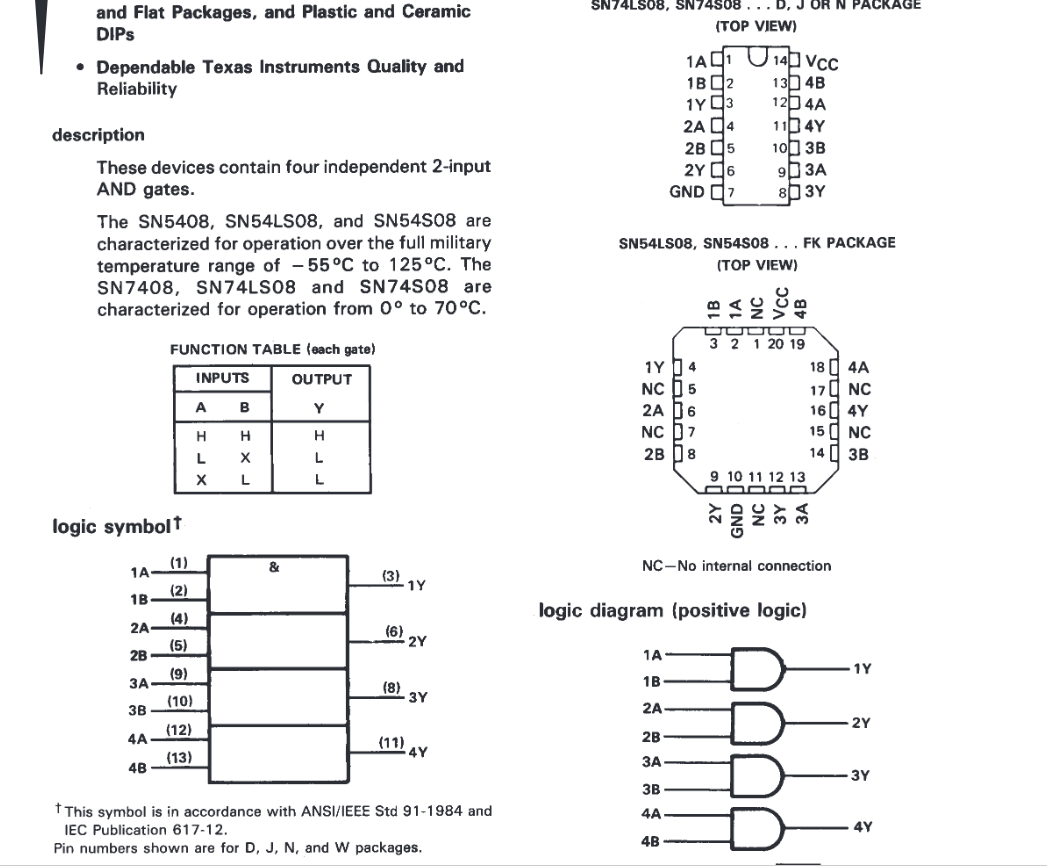
\includegraphics[width=0.7\linewidth]{media/sn74ls08.png}
\section{FPGA~\cite[Section~B.6.5]{stephen2022fundamentals}}
\includegraphics[width=0.5\linewidth]{./media/FPGA.png}
\includegraphics[width=0.5\linewidth]{./media/LUT.png}

% \chapter{Verilog and Schematics}
% \input{labs/01-quartus-setup/body.tex}
% \input{labs/02-verilog-mux/body.tex}
\chapter{Logic minimization}
\maketitle

\section{Logic minimization}

A general optimization criteria for multi-level logic are to Minimize
some combination of:
\begin{enumerate}
\item Area occupied by the logic gates and interconnect;
\item the Critical Path Delay of the longest path through the logic;
\item the Degree of Testability of the circuit, measured in terms of the percentage
of faults covered by a specified set of test vectors, for an appropriate fault model
(Eg., single stuck faults, multiple stuck faults, etc.);
\item Power consumed by the logic gates.
\end{enumerate}

In this course, we will start with two-level multi-input circuits and a criteria
based on the number of gates/transistors/diodes.

\section{Programmable Logic Arrays}
\includegraphics[width=0.5\linewidth]{figures/PLA-abstract.png}
\includegraphics[width=0.5\linewidth]{figures/PLA-logic.png}

\section{Two-level circuits}
The cost that we are going to consider in this class depend upon:
\begin{enumerate}
\item Number of gates.
\item Number of input to the gates.
\end{enumerate}
More gates need more transistors, more area on the chip. More-inputs the gate
need more transistors within each gate. Number of gate inputs can be considered
secondary criterion to the number of gates.

\begin{example}
  Find the cost of the following Boolean expression $X = \bA\bB C + AB\bC + A\bB$.
\end{example}

\begin{prob}[5 marks]
  Find the cost of the following Boolean expression $X = A\bB C + \bA B\bC + \bB
  C$.
\end{prob}

\section{Terminology for K-maps}
Running Example: $f = \sum m(0, 1, 2, 3, 7) = \bx_1 + x_1 x_2 x_3$.
\begin{description}
  \item[Literal] A single variable or its complement. Example: $\bx, x_1, x_2, x_3$
  \item[Implicant] A product term which is true for a function. All minterms are
    implicants. Example: $x_1
    x_2 x_3$, $\bx_1$, $m_0 = \bx_1\bx_2\bx_3$, $\bx_1 x_3$, $\bx_1 \bx_3$.
  \item [Prime Implicant] An implicant that cannot be combined into fewer
    literals. Example: $\bx_1, x_2x_3$.
  \item [Essential Prime Implicant] An implicant that cannot be combined into
    fewer literals. Example: $x_2x_3$.
  \item [Cover] : List of Prime Implicants that account for all $f = 1$.
  \item [Cost]: Number of gates (excluding not gate on literals) and number of
      inputs to each gate.
\end{description}

\begin{example}
  Find minimum cost expression for the function $f(x_1, x_2, x_3) = \prod M(4, 5, 6)$
\end{example}
\vspace{10em}

\begin{prob}[10 marks]
  Find minimum cost expression for the function $f(x_1, x_2, x_3) = \prod M(2, 5, 6)$
\end{prob}
\vspace{10em}

\subsection{Incompletely specified functions or Don't cares}

\begin{figure}[h!]
  \centering
  \begin{circuitikz}
    \draw (0,0) node[seven segment val=0 dot off box on]{};
    \draw (1,0) node[seven segment val=1 dot off box on]{};
    \draw (2,0) node[seven segment val=2 dot off box on]{};
    \draw (3,0) node[seven segment val=3 dot off box on]{};
    \draw (4,0) node[seven segment val=4 dot off box on]{};
    \draw (5,0) node[seven segment val=5 dot off box on]{};
    \draw (6,0) node[seven segment val=6 dot off box on]{};
    \draw (7,0) node[seven segment val=7 dot off box on]{};
    \draw (8,0) node[seven segment val=8 dot off box on]{};
    \draw (9,0) node[seven segment val=9 dot off box on]{};
  \end{circuitikz}\includegraphics[width=0.1\linewidth]{figures/seven_segment.png}
  \caption{7 Segment Representations of Each Integer}
  \label{sevensegs}
\end{figure}

\begin{tabular}{cccc|c}
  \toprule
  \multicolumn{4}{c|}{BCD Value} & LED Segment \\
  $D_3$ & $D_2$ & $D_1$ & $D_0$ & E \\
  \midrule
  0 & 0 & 0 & 0 & 0\\
  0 & 0 & 0 & 1 & 1\\
  0 & 0 & 1 & 0 & 0\\
  0 & 0 & 1 & 1 & 1\\
  0 & 1 & 0 & 0 & 1\\
  0 & 1 & 0 & 1 & 1\\
  0 & 1 & 1 & 0 & 0\\
  0 & 1 & 1 & 1 & 1\\
  1 & 0 & 0 & 0 & 0\\
  1 & 0 & 0 & 1 & 1\\
  1 & 0 & 1 & 0 & d\\
  1 & 0 & 1 & 1 & d\\
  1 & 1 & 0 & 0 & d\\
  1 & 1 & 0 & 1 & d\\
  1 & 1 & 1 & 0 & d\\
  1 & 1 & 1 & 1 & d\\
  \bottomrule
\end{tabular}

\begin{example}
  Find minimum cost expression for the function
  \[ f(x_1, \dots, x_4) = \sum m(2, 4, 5, 6, 10) + D(12, 13, 14, 15) \]
\end{example}
\vspace{10em}

\begin{prob}[10 marks]
  Find minimum cost expression for the function
  \[ f(x_1, \dots, x_4) = \sum m(0, 2, 4, 6, 7, 8, 9, 13) + D(1, 12, 15) \]
\end{prob}
\vspace{10em}


%\maketile
\section{A few more Boolean problems}
\begin{example}
  Simplify the following Boolean expression:
  \[ f = x_1\bx_3 \bx_4 + x_2 \bx_3 \bx_4 + x_1 \bx_2 \bx_3 \]
\end{example}

% \begin{example}
%   Assume that a large room has three doors and that a switch near each door controls a light in the room. It has to be possible to turn the light on or off by changing the state of any one
%   of the switches.\\
%   \includegraphics[width=\linewidth]{figures/design-a-3-way-light-switch.pdf}
% \end{example}


\begin{prob}[20 marks]
A simple security system for two doors consists of a card reader and a keypad.

A person may open a particular door if he or she has a card containing the corresponding code and enters an authorized keypad code for that card. Note that card-code and keypad-code are different. The outputs from the card reader are given in the table below.


To unlock a door, a person must hold down the proper keys on the keypad and, then, insert the card in the reader. The authorized keypad code for door 1 is 10, and the authorized keypad code for door 2 is 11. If the card has an invalid code or if the wrong keypad code is entered, the alarm will ring when the card is inserted. If the correct keypad code is entered, the corresponding door will be unlocked when the card is inserted.

Design the logic circuit for this simple security system. Your circuit’s inputs will consist of a card code AB, and a keypad code CD. The circuit will have three outputs
XYZ (if X is 1, door 1 will be opened; if Y is 1, door 2 will be opened; if Z  1, the alarm will sound).

Find the minimal cost two-level circuit using K-maps for X, Y, Z. Provide the minimal cost. (It can be either of SOP/POS forms)\\
\includegraphics[width=0.5\linewidth]{figures/card-reader-keypad.png}%
\includegraphics[width=0.5\linewidth]{figures/card-reader-table.png}
\end{prob}

\maketitle

%\includegraphics[width=0.3\linewidth]{figures/K-map-flowchart.png}

%
\begin{example}
  \begin{Karnaugh}{AB}{CD}
    \minterms{4,5,6,8,9,10,13}
    \indeterminants{0,7,15}
  \end{Karnaugh}
\end{example}%
% 

\begin{prob}[10 marks]
  Find the minimum SOP (sum of products) and POS (product of sum) expression for
  the function $f(a,b,c,d) = \prod M(5, 7, 13, 14, 15) \cdot \prod D(1, 2, 3, 9)$
\end{prob}%
% 


\begin{prob}
  Read Chapter 2 up to Section 2.7 of Harris and Harris textbook. Write a statement saying that you have read and understood the chapter. [5 marks]
\end{prob}

\begin{prob}
If the Sum of Products (SOP) form for $ \bar{f} = AB\bC+\bA\bB$, then give the Product of Sums (POS) form for
$f$. [10 marks]
\end{prob}

\begin{prob}
Use DeMorgan's Theorem to find $f$  if  $\bar{f} = (A + \bB C)D + EF$. [10 marks]
\end{prob}


\begin{prob}
  For the function $f = AB\bC + BD$,
  \begin{enumerate}
    \item Write the Truth table. [10 marks]
    \item Write $f$ in Sum of Products form. [10 marks]
    \item Write $f$ in canonical minterm form. [10 marks]
    \item Write $f$ as Product of Sums. [10 marks]
    \item Write $f$ in canonical maxterm form. [10 marks]
  \end{enumerate}
\end{prob}

\begin{table}
  \centering
  \begin{tabular}{c|ccc||c}
    \toprule
    Row & $x_1$ & $x_2$ & $x_3$ & f \\
    \midrule
    0 & 0 & 0 & 0 & 0 \\
    1 & 0 & 0 & 1 & 1 \\
    2 & 0 & 1 & 0 & 1 \\
    3 & 0 & 1 & 1 & 0 \\
    4 & 1 & 0 & 0 & 1 \\
    5 & 1 & 0 & 1 & 0 \\
    6 & 1 & 1 & 0 & 0 \\
    7 & 1 & 1 & 1 & 1 \\
    \bottomrule
    \end{tabular}
    \caption{Truth table for a 3-way light switch}
    \label{tab:3-way-light-switch}
\end{table}

\begin{prob}
 Implement the function in Table~\ref{tab:3-way-light-switch} using only NAND
 gates. [10 marks]
\end{prob}

\begin{prob}
 Implement the function in Table~\ref{tab:3-way-light-switch} using only NOR
 gates. [10 marks]
\end{prob}

%\section{Sept 13th Lecture}

\begin{prob}
Find the minimum-cost Sum of Products (SOP) and Product of Sums (POS) forms for the function $f(x_1 , x_2 , x_3 ) =
m(1, 3, 4, 5)$.  Chose the minimum-cost expression by comparing Product of Sums (POS) and Sum of Products (SOP) forms. [10 marks]
\label{prob:237}
\end{prob}

\begin{prob}
Find the minimum-cost Sum of Products (SOP) and Product of Sums (POS) forms for the function $f(x_1 , x_2 , x_3) =
\sum m(1, 5, 7) + D(2, 4)$.  [10 marks]
\end{prob}

\begin{prob}
Find the minimum-cost Sum of Products (SOP) and Product of Sums (POS) forms for the function $f(x_1 , x_2 , x_3,
x_4) = \prod M(1, 2, 4, 5, 7, 8, 9, 10, 12, 14, 15).$  Chose the minimum-cost
expression by comparing Product of Sums (POS) and Sum of Products (SOP) forms. [10 marks]
\end{prob}

\begin{prob}
Find the minimum-cost Sum of Products (SOP) and Product of Sums (POS) forms for the function $f(x_1 , x_2 , x_3, x_4) =
\sum m(2, 8, 9, 12, 15) + D(1, 3, 6, 7).$  Chose the minimum-cost expression
by comparing Product of Sums (POS) and Sum of Products (SOP) forms. [10 marks]
\end{prob}

\begin{prob}
Derive a minimum-cost realization of the four-variable function that is equal to 1 if exactly
two or exactly three of its variables are equal to 1; otherwise it is equal to
0.  [10 marks]
\end{prob}

\begin{prob}
  Find the minimum-cost Sum of Products (SOP) and Product of Sums (POS) forms for the function $f(x_1 , \dots, x_5) =
  \sum m(1, 3, 4, 6, 8, 9, 11, 13, 14, 16, 19, 20, 21, 22, 24, 25) + D(5, 7,
  12, 15, 17, 23).$  Chose the minimum-cost expression by comparing Product of Sums (POS) and Sum of Products (SOP) forms. [10 marks]
\end{prob}

\chapter{Review}


\section{Syllabus covered}

\renewcommand{\done}{\checkmark}
\begin{itemize}
  \item[\done] Binary numbers
  \item[\done] Generate minterms, maxterms, SOP canonical form and POS
    canonical forms and convert between them\\
  \item[\done]  Understand and use the laws and theorems of Boolean Algebra
  \item[\done]  Perform algebraic simplification using Boolean algebra
  \item[\done]  Simplification using K-maps
  \item[\done]  Derive sum of product and product of sums expressions for a combinational circuit
  \item[\done]  Convert combinational logic to NAND-NAND and NOR-NOR forms
  %\item[\done]  Simplification using Quine-McCluskey method, PI tables and Petrick's method
  \item Hexadecimal, Sign-magnitude, One's-complement and
    Two's complement. Conversions between them.
  \item  Design combinational circuits for positive and negative logic
  \item  Design Hazard-free two level circuits and understand Hazards in multi-level circuits
  \item Compute noise margin of one device
  \item Describe how tri-state and open-collector outputs are different from totem-pole outputs.
  \item Different between and limitations of master-slave and edge-triggered flip-flops.
  \item Compute fan out and noise margin of one device driving the same time
  \item Know the differences and similarities between PAL, PLA, and ROMs and can use each for logic design
  \item Design combinational circuits using multiplexers and decoders
  \item Analyze a sequential circuit and derive a state-table and a state-graph
  \item Understand the difference between synchronous and asynchronous inputs
  \item Derive a state graph or state table from a word description of the problem
  \item Reduce the number of states in a state table using row reduction and implication tables
  \item Perform a state assignment using the guideline method
  \item Implement a design using JK, SR, D or T flip-flops
  \item Analyse and design both Mealy and Moore sequential circuits with multiple inputs and multiple outputs
  \item Convert between Mealy and Moore designs
  \item Partition a system into multiple state machines
\end{enumerate}

\subsection{Labs (not questioned in exams)}
\begin{itemize}
  \item Use computer tools to enter designs graphically and HDL
  \item Simulate designs using computer tools
  \item Use computer tools to program gate arrays logic and debug and test
\end{itemize}

\newpage

\chapter{Sample midterm exam}

\maketitle

Student Name: \hfill Student Email: \hspace{10em}
\section{Instructions}
\begin{itemize}
  \item Time allowed is 50 minutes. (This sample exam might be lengthier than the actual exam.  Same instruction will apply to the midterm.)
  \item In order to minimize distraction to your fellow students, you may not leave
  during the last 10 minutes of the examination.
  \item The examination is closed-book. One 8x11in cheatsheet is allowed.
  \item Non-programmable calculators are permitted.
  \item The maximum number of marks is 80, as indicated; the midterm examination
  amounts 10\% toward the final grade.
  \item Please colored pen/pencils for K-maps, use a pen or heavy pencil to ensure legibility.
  \item Please show your work; where appropriate, marks will be awarded for proper and well-reasoned explanations.
\end{itemize}

%\begin{prob}
%  Number conversions:
%  \begin{enumerate}
%    \item Use repeated division to convert $230_{10}$ to octal representation (5 marks).
%    \item What is the value of $19D_{16}$ in base 10 (5 marks).
%    \item A 6-bit two's complement number is $100011_{2}$. Convert it to (signed) decimal (5 marks).
%    \item Represent $-23_{10}$ in two's complement binary notation (5 marks).
%  \end{enumerate}
%\end{prob}

\begin{prob}
  Consider the circuit below\\
  \begin{tikzpicture}[circuit logic US]
    \matrix[column sep=7mm]
    {
      \node (A) {A}; &  &  & \\
      & \node [xor gate] (AxorB) {}; &  &\\
      \node (B) {B}; &  & \node [xor gate] (f) {}; \\
      & \node [xor gate] (BxorC) {}; &  & \\
      \node (C) {$\bC$}; &  & &\\
    };
    \draw (A.east) --++(right:3mm) |- (AxorB.input 1);
    \draw (B.east) --++(right:3mm) |- (AxorB.input 2);
    \draw (A.east) --++(right:1mm) |- (BxorC.input 1);
    \draw (C.east) --++(right:3mm) |- (BxorC.input 2);
    \draw (AxorB.output) to [edge label=$g_1$] ++(right:3mm) |- (f.input 1);
    \draw (BxorC.output) to [edge label=$g_2$] ++(right:3mm) |- (f.input 2);
    \draw (f.output) to [edge label=Y] ++(right:3mm) ;
  \end{tikzpicture} \\
  By algebraic manipulation, prove or disprove that $Y = \bB \bC + B C$ (10 marks).
\end{prob}

\begin{prob}
Use the following 4-variable K-map for F (A, B, C, D), and find
  a minimal sum of products (SOP) expression for F (15 marks)\\
\begin{minipage}{0.5\linewidth}
  \centering
  \begin{Karnaugh}{AB}{CD}
    \minterms{0,1,5,6,7,8,9,14}
    \maxterms{2,3,4,10,11,12,13,15}
  \end{Karnaugh}\\
  %A=0
\end{minipage}%
%\begin{minipage}{0.5\linewidth}
%  \centering
%  \begin{Karnaugh}{BC}{DE}
%    \minterms{1,4,5,6,7,9,12,14}
%  \end{Karnaugh}\\
%  A=1
%\end{minipage}
\end{prob}

\begin{prob}
  Use boolean algebra to find an SOP expression
for Y in the circuit below. Draw an equivalent
  circuit beside the given circuit (5 marks).\\
  \includegraphics[width=0.4\linewidth]{figures/bubble-pushing-circuit.png}
\end{prob}

\begin{prob}
  Consider the function Y given below.
  \[ Y(A, B, C, D) = \sum m(0, 3, 5, 7, 8, 14) + d(2, 12, 15) \]
  \begin{enumerate}
    \item Draw a K-maps to derive a minimum SOP and POS expressions for Y .
      Indicate all essential prime implicants for Y or $\bY$ in your K-maps (20 marks).
    \item Sketch a two-level NOR-NOR circuit for Y. Assume that A, B, C, and D are available in true end complimentary forms (5 marks).
    \item Write Y in Product of sums (POS) \emph{canonical} form (5 marks).
  \end{enumerate}
\end{prob}

\begin{prob}
  Design a minimal SOP circuit to add two two-bit unsigned numbers. Denote the two bits of first number as $A_1A_0$ and the two bits of second number as $B_1B_0$. The result will be a 2-bit sum $S_1S_0$ and a carry $C$. Start with filling out the following truth table (3 example rows are provided) and then use K-maps to find minimal SOP for $S_1$, $S_0$ and a single carry bit $C_1$ (20 marks).\\
  \begin{tabular}{cccc|ccc}
    \toprule
    $A_1$ & $A_0$ & $B_1$ & $B_0$ & $C_1$ & $S_1$ & $S_0$  \\
    \midrule
    0 & 0 & 0 & 0 &   &   &   \\
    0 & 0 & 0 & 1 &   &   &   \\
    0 & 0 & 1 & 0 &   &   &   \\
    0 & 0 & 1 & 1 &   &   &   \\
    0 & 1 & 0 & 0 &   &   &   \\
    0 & 1 & 0 & 1 & 0 & 1 & 0 \\
    0 & 1 & 1 & 0 &   &   &   \\
    0 & 1 & 1 & 1 &   &   &   \\
    1 & 0 & 0 & 0 &   &   &   \\
    1 & 0 & 0 & 1 &   &   &   \\
    1 & 0 & 1 & 0 &   &   &   \\
    1 & 0 & 1 & 1 &   &   &   \\
    1 & 1 & 0 & 0 &   &   &   \\
    1 & 1 & 0 & 1 & 1 & 0 & 0 \\
    1 & 1 & 1 & 0 &   &   &   \\
    1 & 1 & 1 & 1 & 1 & 1 & 0 \\
    \bottomrule
  \end{tabular}
\end{prob}

\chapter{Number System}

\section{Place value number system}

\begin{itemize}
\item What is a place value number system?
\item What are some examples?
\item What are some non-examples?
\item What is a radix (or base)? 
\item How to convert between different radix in place value system?
\item What are some commonly used number systems in computer engineering?
\end{itemize}

\subsection{Decimal number system}

\vspace{15em}
\begin{comment}
A decimal number 1342 can be written as
\begin{align*}
  1342&=1\times1000 + 3\times100 + 4\times10 + 2\times1
        \\
      &=1\times10^3 + 3\times10^2+4\times10^1 + 2\times10^0.
\end{align*}

Decimal numbers are said to be of base (or radix) 10. One can generalize this
idea to arbitrary base (or radix) $r$. The same number expressed in some other
base $r$ will have a very different value:
\begin{align*}
  (1342)_r &=1\times r^3 + 3\times r^2+4\times r^1 + 2\times r^0.
\end{align*}

In general the \emph{value} of a arbitrary $n$-digit number $d_{n-1}d_{n-2}
\dots d_1 d_0$ in base $r$ is:
\begin{align*}
  (d_{n-1}d_{n-2} \dots d_1 d_0)_r &=d_{n-1} \times r^{n-1} + d_{n-2}\times r^{n-2}+ \dots + d_1\times r^1 + d_0\times r^0 &= \sum_{k=0}^{n-1} d_k r^k
\end{align*}
Each digit value is always smaller than base $d_k <= r-1$.
\end{comment}

\subsection{Binary numbers}

\vspace{15em}
\begin{comment}
Numbers with base $2$ are called binary numbers. For example, the number
$(10110)_2$ has value:
\begin{align*}
  (10110)_2 &= 1 \times 2^4+ 0 \times 2^3 + 1\times 2^2 + 1 \times 2^1+ 0\times 2^0
              \\
            &= 22.
\end{align*}
\end{comment}

\subsection{Conversion between different radix}
\begin{example}
  Convert the following binary numbers to decimal: $(11110)_2$, $(100111)_2$.
\end{example}
\vspace{10em}

\paragraph{Conversion from decimal to binary}
The value is in decimal because we find it easy to do calculations in decimal
numbers. Decimal values can be converted back to Binary representation by
\emph{repeated division} by 2 while noting down the remainder. Allow me
to use $/$ sign to denote both quotient and remainder after division. Let's convert $(22)_{10}$
back to binary: 

\begin{align*}
  22 / 2 &= (11, 0) & \text{ 11 is the quotient and 0 is the remainder} \\
  11 / 2 &= (5, 1) & \text{5 is the quotient and 1 is the remainder}\\
  5 / 2 &= (2, 1) & \\ 
  2 / 2 &= (1, 0) & \\
  1 / 2 &= (0, 1) &
\end{align*}

Read the remainders from bottom to top and right them as left to right, to form the resultant binary number $(22)_{10} = (10110)_2$.

\begin{example}
Find the binary representation for decimal numbers: $123$ and $89$. Show your work.
\end{example}
\vspace{10em}


\section{Hexadecimal numbers}
Numbers with base $16$ are called Hexadecimal numbers. From 0 to 9 the symbols
are same as decimal numbers. From 10 to 15, Hexadecimal numbers use A to F.
\[ A = 10, B = 11, C = 12, D = 13, E = 14, F = 15 \]. Example, $(10AD)_{16} = 1
\times 16^3 + 10 \times 16^1 + 13 = 4096 + 160 + 13 = 4269$.

\section{Octal numbers}
Numbers with base $8$ are called octal numbers. Example, $(354)_8 = 3 \times 8^2
+ 5 \times 8 + 4 = 192 + 40 + 4 = 236$.



\section{Hexadecimal/octal to binary and vice-versa}
Normally, if you have to convert between a number of base $r_1$ to a number of
base $r_2$, we will have to convert it via decimal numbers. Convert from base
$r_1$ to decimal and then from decimal to $r_2$.

Since Hexadecimal base $16$ is an exact power of $2$ ($16 = 2^4$). Conversion
between Hexadecimal to binary is easy. You can group 4 binary digits from right
to left and convert each group of 4 binary digits to a single Hexadecimal digit
and back. Example, $(10110)_2 = (0001\_0110)_2 = (16)_{16}$. To convert back.
Take example, $(10AD)_{16} = (0001\_0000\_1010\_1101)_2 = (1\_0000\_1010\_1101)_2$.

\begin{prob}
  Find the binary and decimal values of the following Hexadecimal numbers
  $(A25F)_{16}$, $(F0F0)_{16}$.
\end{prob}
\vspace{10em}



Similarly octal to binary can proceed by grouping 3-binary digits at a time.
Example, $(354)_8 = (011\_101\_100)_2$.

\begin{prob}
  Find the binary and decimal values of the following Octal numbers
  $(3751)_8$ and $(722)_8$.
\end{prob}
\vspace{10em}

\input{./0831-number-system/0902-notes.tex}
Always show your work/process. Correct final answer is worth less than the
correct process. Submit digitally via brightspace.

\begin{prob}
  Convert the each of the following numbers into binary, decimal, hexadecimal,
octal numbers. Show your work. Just filling in the values is not enough. ($8 \times 6 $ marks)

  \begin{tabular}{lllll}
    \toprule
     & Binary & Decimal & Hexadecimal & Octal \\
    \midrule
    a)& $1010_2$     &   &   &    \\
    b)& $10\_0110_2$ &   &   &   \\
    c)&   & $329_{10}$   &   &   \\
    d)&   & $741_{10}$   &   &   \\
    e)&   &   & $7D_{16}$    &   \\
    f)&   &   & $EC3A_{16}$  &   \\
    g)&   &   &   & $351_8$\\
    h)&   &   &   & $2563_8$\\
    \bottomrule
  \end{tabular}
\end{prob}

\vspace{20em}

\begin{prob}
  Convert the each of the following numbers into decimal, 8-bit sign-magnitude binary,
  8-bit one's complement binary and 8-bit two's complement binary. Show your work. ($6 \times 6 $ marks)

  \begin{tabular}{lllll}
    \toprule
    & Decimal & Sign-magnitude & One's complement & Two's complement \\
    \midrule
    a) & $-79_{10}$ & & & \\
    b) & $-110_{10}$ & & & \\
    c) & & & & $0110\_1110_2$ \\
    d) & &  & & $1011\_1101_2$\\
    e) & & & $0110\_1101_2$&  \\
    f) & &  & $1001\_1010_2$& \\
    \bottomrule
  \end{tabular}
\end{prob}

\vspace{20em}

\begin{prob}
  Convert the decimal numbers to 6-bit two's complement binary and then add
  them. Check if the addition causes overflow ($3 \times 6$ marks).
  \begin{enumerate}
  \item $-16_{10} - 7_{10}$
  \item $19_{10} - 5_{10}$
  \item $-4_{10} - 29_{10}$
  \end{enumerate}
\end{prob}

\vspace{20em}

\begin{prob}
  \begin{enumerate}
  \item Convert $299_{10}$  to binary coded decimal (BCD). (2 marks)
  \item Convert $1001\_ 0111\_ 0101_{BCD}$  to decimal. (2 marks)
  \item Convert $0110\_ 1101_{BCD}$  to binary. (4 marks)
  \end{enumerate}
\end{prob}

\vspace{20em}

\chapter{Adders, Muxes and Decoders}

% \section{FPGA~\cite[Section~B.6.5]{stephen2022fundamentals}}
% 
% \includegraphics[width=0.5\linewidth]{./media/FPGA.png}
% \includegraphics[width=0.5\linewidth]{./media/LUT.png}\\
% \includegraphics[width=0.5\linewidth]{./media/FF-LUT.png}
% \includegraphics[width=0.5\linewidth]{./media/programmed-FPGA.png}
% 
% 
% \begin{definition}[Random Access Memory (RAM)] Structure of a RAM is as follows:\\
%   \includegraphics[width=0.3\linewidth]{./media/memory-array.png}
%   \includegraphics[width=0.3\linewidth]{./media/memory-array-32kb.png}
%   \includegraphics[width=0.3\linewidth]{./media/SRAM-cell.png}\\
%   \includegraphics[width=0.7\linewidth]{./media/SRAM.png}
% \end{definition}
% 
% \begin{definition}[Read Only Memory (ROM)] Structure of a ROM is as follows:\\
%   \includegraphics[width=\linewidth]{./media/rom.png}
% \end{definition}


\begin{definition}[Fan-in]
  The fan-in of a logic gate is number of  inputs to a logic gate.~\cite[Section~B.8.9]{stephen2022fundamentals}
\end{definition}
\includegraphics[width=0.3\linewidth]{./media/fan-in.png}

\begin{remark}[Fan-in]
  The fan-in of a gate is limited by the propagation delay $t_p$. Higher the
  fan-in, higher the $t_p$. The output
  voltage thresholds like $V_{OL}$ and $V_{OH}$ also limit fan-in. Higher the
  fan-in, higher is $V_{OL}$ (and lower is the $V_{OH}$).
\end{remark}

\begin{example}
  Implement an OR gate with fan-in of 7 using OR gates with fan-in of 3.
\end{example}
\vspace{5em}

\begin{definition}[Fan-out]
  The fan-out of a logic gate is the maximum number of other gates that can be connected
  to output of a gate.~\cite[Section~B.8.9]{stephen2022fundamentals}
\end{definition}
\includegraphics[width=0.5\linewidth]{./media/fan-out.png}

% \begin{definition}[Programmable Logic Array (PLA) ] Structure of a PLA:\\
%   \includegraphics[width=0.7\linewidth]{./media/AND-OR-PLA.png}~\cite[Section~B.6.1]{stephen2022fundamentals}
%   %\includegraphics[width=0.7\linewidth]{./media/NOR-NOR-PLA.png}
% \end{definition}
% 
% \begin{definition}[Programmable Array Logic (PAL)] Structure of a PAL:\\
%   \includegraphics[width=0.7\linewidth]{./media/AND-OR-PAL.png}~\cite[Section~B.6.2]{stephen2022fundamentals}
% \end{definition}
% 
% \begin{example}
%   What is the difference between PLA and PAL?
% \end{example}
% \vspace{5em}

\section{Timing parameters for sequential circuit~\cite[Section~3.5]{harris2022digital}}

\includegraphics[width=0.6\linewidth]{./media/ff-timings.png}\\
\begin{definition}[Setup time $t_{su}$ of a latch/flip-flop]
  Time for which input must be stable before the clock edge.
\end{definition}

\begin{definition}[Hold time $t_h$ of a latch/flip-flop]
  Time for which input must be stable after the clock edge.
\end{definition}

\begin{definition}[Clock-to-Q contamination delay $t_{ccq}$ of a latch/flip-flop]
  Time taken to influence (contaminate) the Q output after the clock edge.
\end{definition}

\begin{definition}[Clock-to-Q propagation delay $t_{ccq}$ of a latch/flip-flop]
  Time taken for Q output to stabalize  after the clock edge.
\end{definition}
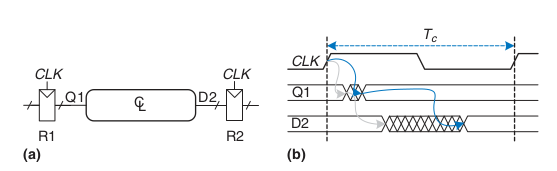
\includegraphics[width=0.8\linewidth]{./media/fig3.38.png}

\begin{definition}[Setup Time Constraint]
  $T_c > t_{pcq} + t_{pd} + t_{setup}$\\
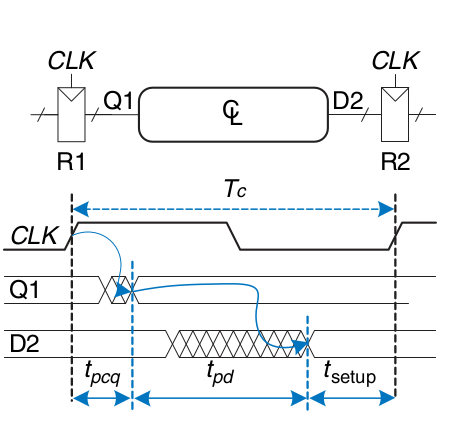
\includegraphics[width=0.8\linewidth]{./media/fig3.39.png}
\end{definition}

\begin{definition}[Hold Time Constraint]
  $t_{ccq} + t_{cd} \ge t_{hold}$\\
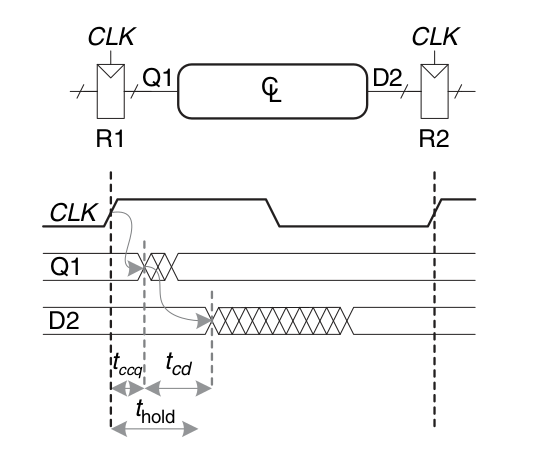
\includegraphics[width=0.8\linewidth]{./media/fig3.40.png}
\end{definition}


\chapter{Sequential Logic}

% \section{FPGA~\cite[Section~B.6.5]{stephen2022fundamentals}}
% 
% \includegraphics[width=0.5\linewidth]{./media/FPGA.png}
% \includegraphics[width=0.5\linewidth]{./media/LUT.png}\\
% \includegraphics[width=0.5\linewidth]{./media/FF-LUT.png}
% \includegraphics[width=0.5\linewidth]{./media/programmed-FPGA.png}
% 
% 
% \begin{definition}[Random Access Memory (RAM)] Structure of a RAM is as follows:\\
%   \includegraphics[width=0.3\linewidth]{./media/memory-array.png}
%   \includegraphics[width=0.3\linewidth]{./media/memory-array-32kb.png}
%   \includegraphics[width=0.3\linewidth]{./media/SRAM-cell.png}\\
%   \includegraphics[width=0.7\linewidth]{./media/SRAM.png}
% \end{definition}
% 
% \begin{definition}[Read Only Memory (ROM)] Structure of a ROM is as follows:\\
%   \includegraphics[width=\linewidth]{./media/rom.png}
% \end{definition}


\begin{definition}[Fan-in]
  The fan-in of a logic gate is number of  inputs to a logic gate.~\cite[Section~B.8.9]{stephen2022fundamentals}
\end{definition}
\includegraphics[width=0.3\linewidth]{./media/fan-in.png}

\begin{remark}[Fan-in]
  The fan-in of a gate is limited by the propagation delay $t_p$. Higher the
  fan-in, higher the $t_p$. The output
  voltage thresholds like $V_{OL}$ and $V_{OH}$ also limit fan-in. Higher the
  fan-in, higher is $V_{OL}$ (and lower is the $V_{OH}$).
\end{remark}

\begin{example}
  Implement an OR gate with fan-in of 7 using OR gates with fan-in of 3.
\end{example}
\vspace{5em}

\begin{definition}[Fan-out]
  The fan-out of a logic gate is the maximum number of other gates that can be connected
  to output of a gate.~\cite[Section~B.8.9]{stephen2022fundamentals}
\end{definition}
\includegraphics[width=0.5\linewidth]{./media/fan-out.png}

% \begin{definition}[Programmable Logic Array (PLA) ] Structure of a PLA:\\
%   \includegraphics[width=0.7\linewidth]{./media/AND-OR-PLA.png}~\cite[Section~B.6.1]{stephen2022fundamentals}
%   %\includegraphics[width=0.7\linewidth]{./media/NOR-NOR-PLA.png}
% \end{definition}
% 
% \begin{definition}[Programmable Array Logic (PAL)] Structure of a PAL:\\
%   \includegraphics[width=0.7\linewidth]{./media/AND-OR-PAL.png}~\cite[Section~B.6.2]{stephen2022fundamentals}
% \end{definition}
% 
% \begin{example}
%   What is the difference between PLA and PAL?
% \end{example}
% \vspace{5em}

\section{Timing parameters for sequential circuit~\cite[Section~3.5]{harris2022digital}}

\includegraphics[width=0.6\linewidth]{./media/ff-timings.png}\\
\begin{definition}[Setup time $t_{su}$ of a latch/flip-flop]
  Time for which input must be stable before the clock edge.
\end{definition}

\begin{definition}[Hold time $t_h$ of a latch/flip-flop]
  Time for which input must be stable after the clock edge.
\end{definition}

\begin{definition}[Clock-to-Q contamination delay $t_{ccq}$ of a latch/flip-flop]
  Time taken to influence (contaminate) the Q output after the clock edge.
\end{definition}

\begin{definition}[Clock-to-Q propagation delay $t_{ccq}$ of a latch/flip-flop]
  Time taken for Q output to stabalize  after the clock edge.
\end{definition}
\includegraphics[width=0.8\linewidth]{./media/fig3.38.png}

\begin{definition}[Setup Time Constraint]
  $T_c > t_{pcq} + t_{pd} + t_{setup}$\\
\includegraphics[width=0.8\linewidth]{./media/fig3.39.png}
\end{definition}

\begin{definition}[Hold Time Constraint]
  $t_{ccq} + t_{cd} \ge t_{hold}$\\
\includegraphics[width=0.8\linewidth]{./media/fig3.40.png}
\end{definition}


% %\chapter{Review 2}
% %\input{./1031-review/1031-syllabus-covered.tex}
% %\input{./1031-review/20221109-midterm.tex}
\section{Mealy Moore Sequence detector}

% \section{FPGA~\cite[Section~B.6.5]{stephen2022fundamentals}}
% 
% \includegraphics[width=0.5\linewidth]{./media/FPGA.png}
% \includegraphics[width=0.5\linewidth]{./media/LUT.png}\\
% \includegraphics[width=0.5\linewidth]{./media/FF-LUT.png}
% \includegraphics[width=0.5\linewidth]{./media/programmed-FPGA.png}
% 
% 
% \begin{definition}[Random Access Memory (RAM)] Structure of a RAM is as follows:\\
%   \includegraphics[width=0.3\linewidth]{./media/memory-array.png}
%   \includegraphics[width=0.3\linewidth]{./media/memory-array-32kb.png}
%   \includegraphics[width=0.3\linewidth]{./media/SRAM-cell.png}\\
%   \includegraphics[width=0.7\linewidth]{./media/SRAM.png}
% \end{definition}
% 
% \begin{definition}[Read Only Memory (ROM)] Structure of a ROM is as follows:\\
%   \includegraphics[width=\linewidth]{./media/rom.png}
% \end{definition}


\begin{definition}[Fan-in]
  The fan-in of a logic gate is number of  inputs to a logic gate.~\cite[Section~B.8.9]{stephen2022fundamentals}
\end{definition}
\includegraphics[width=0.3\linewidth]{./media/fan-in.png}

\begin{remark}[Fan-in]
  The fan-in of a gate is limited by the propagation delay $t_p$. Higher the
  fan-in, higher the $t_p$. The output
  voltage thresholds like $V_{OL}$ and $V_{OH}$ also limit fan-in. Higher the
  fan-in, higher is $V_{OL}$ (and lower is the $V_{OH}$).
\end{remark}

\begin{example}
  Implement an OR gate with fan-in of 7 using OR gates with fan-in of 3.
\end{example}
\vspace{5em}

\begin{definition}[Fan-out]
  The fan-out of a logic gate is the maximum number of other gates that can be connected
  to output of a gate.~\cite[Section~B.8.9]{stephen2022fundamentals}
\end{definition}
\includegraphics[width=0.5\linewidth]{./media/fan-out.png}

% \begin{definition}[Programmable Logic Array (PLA) ] Structure of a PLA:\\
%   \includegraphics[width=0.7\linewidth]{./media/AND-OR-PLA.png}~\cite[Section~B.6.1]{stephen2022fundamentals}
%   %\includegraphics[width=0.7\linewidth]{./media/NOR-NOR-PLA.png}
% \end{definition}
% 
% \begin{definition}[Programmable Array Logic (PAL)] Structure of a PAL:\\
%   \includegraphics[width=0.7\linewidth]{./media/AND-OR-PAL.png}~\cite[Section~B.6.2]{stephen2022fundamentals}
% \end{definition}
% 
% \begin{example}
%   What is the difference between PLA and PAL?
% \end{example}
% \vspace{5em}

\section{Timing parameters for sequential circuit~\cite[Section~3.5]{harris2022digital}}

\includegraphics[width=0.6\linewidth]{./media/ff-timings.png}\\
\begin{definition}[Setup time $t_{su}$ of a latch/flip-flop]
  Time for which input must be stable before the clock edge.
\end{definition}

\begin{definition}[Hold time $t_h$ of a latch/flip-flop]
  Time for which input must be stable after the clock edge.
\end{definition}

\begin{definition}[Clock-to-Q contamination delay $t_{ccq}$ of a latch/flip-flop]
  Time taken to influence (contaminate) the Q output after the clock edge.
\end{definition}

\begin{definition}[Clock-to-Q propagation delay $t_{ccq}$ of a latch/flip-flop]
  Time taken for Q output to stabalize  after the clock edge.
\end{definition}
\includegraphics[width=0.8\linewidth]{./media/fig3.38.png}

\begin{definition}[Setup Time Constraint]
  $T_c > t_{pcq} + t_{pd} + t_{setup}$\\
\includegraphics[width=0.8\linewidth]{./media/fig3.39.png}
\end{definition}

\begin{definition}[Hold Time Constraint]
  $t_{ccq} + t_{cd} \ge t_{hold}$\\
\includegraphics[width=0.8\linewidth]{./media/fig3.40.png}
\end{definition}


\section{Finite State Machine Optimization}

% \section{FPGA~\cite[Section~B.6.5]{stephen2022fundamentals}}
% 
% \includegraphics[width=0.5\linewidth]{./media/FPGA.png}
% \includegraphics[width=0.5\linewidth]{./media/LUT.png}\\
% \includegraphics[width=0.5\linewidth]{./media/FF-LUT.png}
% \includegraphics[width=0.5\linewidth]{./media/programmed-FPGA.png}
% 
% 
% \begin{definition}[Random Access Memory (RAM)] Structure of a RAM is as follows:\\
%   \includegraphics[width=0.3\linewidth]{./media/memory-array.png}
%   \includegraphics[width=0.3\linewidth]{./media/memory-array-32kb.png}
%   \includegraphics[width=0.3\linewidth]{./media/SRAM-cell.png}\\
%   \includegraphics[width=0.7\linewidth]{./media/SRAM.png}
% \end{definition}
% 
% \begin{definition}[Read Only Memory (ROM)] Structure of a ROM is as follows:\\
%   \includegraphics[width=\linewidth]{./media/rom.png}
% \end{definition}


\begin{definition}[Fan-in]
  The fan-in of a logic gate is number of  inputs to a logic gate.~\cite[Section~B.8.9]{stephen2022fundamentals}
\end{definition}
\includegraphics[width=0.3\linewidth]{./media/fan-in.png}

\begin{remark}[Fan-in]
  The fan-in of a gate is limited by the propagation delay $t_p$. Higher the
  fan-in, higher the $t_p$. The output
  voltage thresholds like $V_{OL}$ and $V_{OH}$ also limit fan-in. Higher the
  fan-in, higher is $V_{OL}$ (and lower is the $V_{OH}$).
\end{remark}

\begin{example}
  Implement an OR gate with fan-in of 7 using OR gates with fan-in of 3.
\end{example}
\vspace{5em}

\begin{definition}[Fan-out]
  The fan-out of a logic gate is the maximum number of other gates that can be connected
  to output of a gate.~\cite[Section~B.8.9]{stephen2022fundamentals}
\end{definition}
\includegraphics[width=0.5\linewidth]{./media/fan-out.png}

% \begin{definition}[Programmable Logic Array (PLA) ] Structure of a PLA:\\
%   \includegraphics[width=0.7\linewidth]{./media/AND-OR-PLA.png}~\cite[Section~B.6.1]{stephen2022fundamentals}
%   %\includegraphics[width=0.7\linewidth]{./media/NOR-NOR-PLA.png}
% \end{definition}
% 
% \begin{definition}[Programmable Array Logic (PAL)] Structure of a PAL:\\
%   \includegraphics[width=0.7\linewidth]{./media/AND-OR-PAL.png}~\cite[Section~B.6.2]{stephen2022fundamentals}
% \end{definition}
% 
% \begin{example}
%   What is the difference between PLA and PAL?
% \end{example}
% \vspace{5em}

\section{Timing parameters for sequential circuit~\cite[Section~3.5]{harris2022digital}}

\includegraphics[width=0.6\linewidth]{./media/ff-timings.png}\\
\begin{definition}[Setup time $t_{su}$ of a latch/flip-flop]
  Time for which input must be stable before the clock edge.
\end{definition}

\begin{definition}[Hold time $t_h$ of a latch/flip-flop]
  Time for which input must be stable after the clock edge.
\end{definition}

\begin{definition}[Clock-to-Q contamination delay $t_{ccq}$ of a latch/flip-flop]
  Time taken to influence (contaminate) the Q output after the clock edge.
\end{definition}

\begin{definition}[Clock-to-Q propagation delay $t_{ccq}$ of a latch/flip-flop]
  Time taken for Q output to stabalize  after the clock edge.
\end{definition}
\includegraphics[width=0.8\linewidth]{./media/fig3.38.png}

\begin{definition}[Setup Time Constraint]
  $T_c > t_{pcq} + t_{pd} + t_{setup}$\\
\includegraphics[width=0.8\linewidth]{./media/fig3.39.png}
\end{definition}

\begin{definition}[Hold Time Constraint]
  $t_{ccq} + t_{cd} \ge t_{hold}$\\
\includegraphics[width=0.8\linewidth]{./media/fig3.40.png}
\end{definition}


% %\input{./1205-mux-decoder/2023-12-01-syllabus-covered.tex}
% \chapter{More definitions}
% 
% \section{FPGA~\cite[Section~B.6.5]{stephen2022fundamentals}}
% 
% \includegraphics[width=0.5\linewidth]{./media/FPGA.png}
% \includegraphics[width=0.5\linewidth]{./media/LUT.png}\\
% \includegraphics[width=0.5\linewidth]{./media/FF-LUT.png}
% \includegraphics[width=0.5\linewidth]{./media/programmed-FPGA.png}
% 
% 
% \begin{definition}[Random Access Memory (RAM)] Structure of a RAM is as follows:\\
%   \includegraphics[width=0.3\linewidth]{./media/memory-array.png}
%   \includegraphics[width=0.3\linewidth]{./media/memory-array-32kb.png}
%   \includegraphics[width=0.3\linewidth]{./media/SRAM-cell.png}\\
%   \includegraphics[width=0.7\linewidth]{./media/SRAM.png}
% \end{definition}
% 
% \begin{definition}[Read Only Memory (ROM)] Structure of a ROM is as follows:\\
%   \includegraphics[width=\linewidth]{./media/rom.png}
% \end{definition}


\begin{definition}[Fan-in]
  The fan-in of a logic gate is number of  inputs to a logic gate.~\cite[Section~B.8.9]{stephen2022fundamentals}
\end{definition}
\includegraphics[width=0.3\linewidth]{./media/fan-in.png}

\begin{remark}[Fan-in]
  The fan-in of a gate is limited by the propagation delay $t_p$. Higher the
  fan-in, higher the $t_p$. The output
  voltage thresholds like $V_{OL}$ and $V_{OH}$ also limit fan-in. Higher the
  fan-in, higher is $V_{OL}$ (and lower is the $V_{OH}$).
\end{remark}

\begin{example}
  Implement an OR gate with fan-in of 7 using OR gates with fan-in of 3.
\end{example}
\vspace{5em}

\begin{definition}[Fan-out]
  The fan-out of a logic gate is the maximum number of other gates that can be connected
  to output of a gate.~\cite[Section~B.8.9]{stephen2022fundamentals}
\end{definition}
\includegraphics[width=0.5\linewidth]{./media/fan-out.png}

% \begin{definition}[Programmable Logic Array (PLA) ] Structure of a PLA:\\
%   \includegraphics[width=0.7\linewidth]{./media/AND-OR-PLA.png}~\cite[Section~B.6.1]{stephen2022fundamentals}
%   %\includegraphics[width=0.7\linewidth]{./media/NOR-NOR-PLA.png}
% \end{definition}
% 
% \begin{definition}[Programmable Array Logic (PAL)] Structure of a PAL:\\
%   \includegraphics[width=0.7\linewidth]{./media/AND-OR-PAL.png}~\cite[Section~B.6.2]{stephen2022fundamentals}
% \end{definition}
% 
% \begin{example}
%   What is the difference between PLA and PAL?
% \end{example}
% \vspace{5em}

\section{Timing parameters for sequential circuit~\cite[Section~3.5]{harris2022digital}}

\includegraphics[width=0.6\linewidth]{./media/ff-timings.png}\\
\begin{definition}[Setup time $t_{su}$ of a latch/flip-flop]
  Time for which input must be stable before the clock edge.
\end{definition}

\begin{definition}[Hold time $t_h$ of a latch/flip-flop]
  Time for which input must be stable after the clock edge.
\end{definition}

\begin{definition}[Clock-to-Q contamination delay $t_{ccq}$ of a latch/flip-flop]
  Time taken to influence (contaminate) the Q output after the clock edge.
\end{definition}

\begin{definition}[Clock-to-Q propagation delay $t_{ccq}$ of a latch/flip-flop]
  Time taken for Q output to stabalize  after the clock edge.
\end{definition}
\includegraphics[width=0.8\linewidth]{./media/fig3.38.png}

\begin{definition}[Setup Time Constraint]
  $T_c > t_{pcq} + t_{pd} + t_{setup}$\\
\includegraphics[width=0.8\linewidth]{./media/fig3.39.png}
\end{definition}

\begin{definition}[Hold Time Constraint]
  $t_{ccq} + t_{cd} \ge t_{hold}$\\
\includegraphics[width=0.8\linewidth]{./media/fig3.40.png}
\end{definition}


% \chapter{Quine McCluskey}
% \input{./0928-quine-mccluskey/0928-nand-nor-gates.tex}
% \section{PI Table reduction and Petrick's method}
This is not in the text-book. For additional reading, please refer to the linked resources on the website.
\\
\includegraphics[width=0.7\linewidth]{1952-quine.png}\\
\includegraphics[width=0.7\linewidth]{1956-mccluskey.png}


\begin{definition}[Implicant]
  Given a function $f$ of $n$ variables, a product term $P$ is an implicant of $f$
  if and only if for every combination of values of the $n$ variables for which $P=1$, $f$ is
  also equal to 1.
\end{definition}

\begin{definition}[Prime Implicant]
  A prime implicant of a function $f$ is an implicant which is no longer an
  implicant if any literal is removed from it.
\end{definition}

There are 4 main steps in the Quine-McCluskey algorithm/PI Table reduction and Petrick's method:

\begin{enumerate}
\item Generate Prime Implicants
\item Construct Prime Implicant Table. PIs as columns, and minterms as
  rows (don't cares are excluded).
\item Reduce Prime Implicant Table by repeating following steps until they
  it cannot be reduced further
\begin{enumerate}
  \item Remove Essential Prime Implicants
  \item Row Dominance: Remove \emph{dominating} rows. (i.e. unnecessary minterms)
  \item Column Dominance: Remove \emph{dominated} columns. (i.e. remove unnecessary PIs)
\end{enumerate}
\item Solve Prime Implicant Table by Petrick's method
\end{enumerate}


\subsection{Generate Prime Implicants}

\begin{example}
  Generate prime implicants of the function 
  \[ F (A, B, C, D) = \sum m(0, 2, 4, 6, 7,
  8, 10, 12, 13, 14, 16, 18, 19, 29, 30)\]
  using Quine-McCluskey method
\end{example}
\includegraphics[width=0.9\linewidth]{1956-mccluskey-table-2.png}

Steps:
\begin{enumerate}
  \item Start with writing minterms in binary format (include don't cares as minterms).
  \item Create potential groups of minterms that can be combined (merged). The only
    minterms that can be combined differ only be single 1. Create a new list of
    combined minterms as n-1 literal implicants.
  \item Check off the minterms that could be combined. Unchecked minterms are
    prime implicants (PIs).
  \item Repeat the grouping process with n-1 literal implicants.
\end{enumerate}

% \begin{prob}
%   Generate PIs for the function $ F(A, B, C, D) = \sum m(0, 2, 3, 4, 5, 6, 7, 8,
%   9, 10, 11, 12, 13)$.
% \end{prob}

\subsection{Prime Implicants table and reduction}

\begin{example}
  Reduce the prime implicants $\{ \bB \bD, C\bD, BD, BC, A\bD, AB \}$ using prime
  implicants table.
\end{example}
\vspace{20em}

\begin{example}
  \begin{Karnaugh}{AB}{CD}
    \minterms{0,4,5,13,15,11}
    \maxterms{1,2,3,6,7,8,9,10,12,14}
    \implicant{0}{4}{red}
    \implicant{4}{5}{blue}
    \implicant{5}{13}{green}
    \implicant{13}{15}{cyan}
    \implicant{15}{11}{orange}
  \end{Karnaugh}
\end{example}
\vspace{10em}

\begin{example}
  \begin{Karnaugh}{AB}{CD}
    \minterms{1,2,3,5,7}
    \indeterminants{0,6,9,13}
    \maxterms{4,8,10,11,12,14,15}
    \implicant{0}{2}{red}
    \implicant{1}{7}{blue}
    \implicant{1}{6}{green}
    \implicant{1}{9}{cyan}
  \end{Karnaugh}
\end{example}
\vspace{10em}

\begin{example}
  Reduce the following PI table\\
  \begin{tabular}{r|ccccccccc}
    \toprule
    & $\bA\bD$ & $\bB\bD$ & $\bC\bD$ & $\bA C$ & $\bB C$ & $\bA B$ & $B \bC$& $A\bB$ & $A \bC$ \\
    \midrule
     0 & X & X & X &   &   &   &   &   &   \\
     2 & X & X &   & X & X &   &   &   &   \\
     3 &   &   &   & X & X &   &   &   &   \\
     4 & X &   & X &   &   & X & X &   &   \\
     5 &   &   &   &   &   & X & X &   &   \\
     6 & X &   &   & X &   & X &   &   &   \\
     7 &   &   &   & X &   & X &   &   &   \\
     8 &   & X & X &   &   &   &   & X & X \\
     9 &   &   &   &   &   &   &   & X & X \\
    10 &   & X &   &   & X &   &   & X &   \\
    11 &   &   &   &   & X &   &   & X &   \\
    12 &   &   & X &   & X &   & X &   & X \\
    13 &   &   &   &   &   &   & X &   & X \\
    \bottomrule
  \end{tabular}
\end{example}
\vspace{20em}
\begin{example}
  \includegraphics[width=\linewidth]{1956-mccluskey-table-4.png}
\end{example}

\subsection{Petrick's method}

\begin{example}
  Solve the Prime Implicant table using Petrick's method\\
  \begin{tabular}{r|cccccc}
    \toprule
    & $p_1 = \bA C$ & $p_2 = \bB C$ & $p_3 = \bA B$ & $p_4 = B \bC$& $p_5 = A\bB$ & $p_6 = A \bC$ \\
    \midrule
     3 & X & X &   &   &   &   \\
     5 &   &   & X & X &   &   \\
     7 & X &   & X &   &   &   \\
     9 &   &   &   &   & X & X \\
    11 &   & X &   &   & X &   \\
    13 &   &   &   & X &   & X \\
    \bottomrule
  \end{tabular}
\end{example}
\vspace{20em}


% \begin{example}
%   Find the minimum SOP expression for the function $F (A, B, C, D) = \sum m(2, 3, 7,
%   9, 11, 13) + \sum d(1, 10, 15)$ using Quine-McCluskey method.
% \end{example}

\chapter{Analog details}

% \section{FPGA~\cite[Section~B.6.5]{stephen2022fundamentals}}
% 
% \includegraphics[width=0.5\linewidth]{./media/FPGA.png}
% \includegraphics[width=0.5\linewidth]{./media/LUT.png}\\
% \includegraphics[width=0.5\linewidth]{./media/FF-LUT.png}
% \includegraphics[width=0.5\linewidth]{./media/programmed-FPGA.png}
% 
% 
% \begin{definition}[Random Access Memory (RAM)] Structure of a RAM is as follows:\\
%   \includegraphics[width=0.3\linewidth]{./media/memory-array.png}
%   \includegraphics[width=0.3\linewidth]{./media/memory-array-32kb.png}
%   \includegraphics[width=0.3\linewidth]{./media/SRAM-cell.png}\\
%   \includegraphics[width=0.7\linewidth]{./media/SRAM.png}
% \end{definition}
% 
% \begin{definition}[Read Only Memory (ROM)] Structure of a ROM is as follows:\\
%   \includegraphics[width=\linewidth]{./media/rom.png}
% \end{definition}


\begin{definition}[Fan-in]
  The fan-in of a logic gate is number of  inputs to a logic gate.~\cite[Section~B.8.9]{stephen2022fundamentals}
\end{definition}
\includegraphics[width=0.3\linewidth]{./media/fan-in.png}

\begin{remark}[Fan-in]
  The fan-in of a gate is limited by the propagation delay $t_p$. Higher the
  fan-in, higher the $t_p$. The output
  voltage thresholds like $V_{OL}$ and $V_{OH}$ also limit fan-in. Higher the
  fan-in, higher is $V_{OL}$ (and lower is the $V_{OH}$).
\end{remark}

\begin{example}
  Implement an OR gate with fan-in of 7 using OR gates with fan-in of 3.
\end{example}
\vspace{5em}

\begin{definition}[Fan-out]
  The fan-out of a logic gate is the maximum number of other gates that can be connected
  to output of a gate.~\cite[Section~B.8.9]{stephen2022fundamentals}
\end{definition}
\includegraphics[width=0.5\linewidth]{./media/fan-out.png}

% \begin{definition}[Programmable Logic Array (PLA) ] Structure of a PLA:\\
%   \includegraphics[width=0.7\linewidth]{./media/AND-OR-PLA.png}~\cite[Section~B.6.1]{stephen2022fundamentals}
%   %\includegraphics[width=0.7\linewidth]{./media/NOR-NOR-PLA.png}
% \end{definition}
% 
% \begin{definition}[Programmable Array Logic (PAL)] Structure of a PAL:\\
%   \includegraphics[width=0.7\linewidth]{./media/AND-OR-PAL.png}~\cite[Section~B.6.2]{stephen2022fundamentals}
% \end{definition}
% 
% \begin{example}
%   What is the difference between PLA and PAL?
% \end{example}
% \vspace{5em}

\section{Timing parameters for sequential circuit~\cite[Section~3.5]{harris2022digital}}

\includegraphics[width=0.6\linewidth]{./media/ff-timings.png}\\
\begin{definition}[Setup time $t_{su}$ of a latch/flip-flop]
  Time for which input must be stable before the clock edge.
\end{definition}

\begin{definition}[Hold time $t_h$ of a latch/flip-flop]
  Time for which input must be stable after the clock edge.
\end{definition}

\begin{definition}[Clock-to-Q contamination delay $t_{ccq}$ of a latch/flip-flop]
  Time taken to influence (contaminate) the Q output after the clock edge.
\end{definition}

\begin{definition}[Clock-to-Q propagation delay $t_{ccq}$ of a latch/flip-flop]
  Time taken for Q output to stabalize  after the clock edge.
\end{definition}
\includegraphics[width=0.8\linewidth]{./media/fig3.38.png}

\begin{definition}[Setup Time Constraint]
  $T_c > t_{pcq} + t_{pd} + t_{setup}$\\
\includegraphics[width=0.8\linewidth]{./media/fig3.39.png}
\end{definition}

\begin{definition}[Hold Time Constraint]
  $t_{ccq} + t_{cd} \ge t_{hold}$\\
\includegraphics[width=0.8\linewidth]{./media/fig3.40.png}
\end{definition}



\bibliography{1130-FSM-optimization/main.bib}
\bibliographystyle{plain}
\end{document}
